% (c)~2012 Dimitrios Vrettos - d.vrettos@gmail.com
\section{Esercizi}
\subsection{Esercizi dei singoli paragrafi}
\subsubsection*{3.2 - Frazioni}

\begin{esercizio}[\Ast]
\label{ese:3.1}
Da un cartoncino rettangolare quadrettato di lati rispettivamente~5 unità e~8~unità viene ritagliata
la forma colorata in grigio, come mostrato nella figura di seguito riportata.
\begin{center}
 % (c) 2012 Dimitrios Vrettos - d.vrettos@gmail.com
% Esercizio 3.1

\begin{tikzpicture}
\draw[step=5mm, black] (0,0) grid (40mm,25mm);

\fill[gray, opacity=.4] (10mm,5mm) rectangle (15mm,10mm);
\fill[gray, opacity=.4] (25mm,5mm) rectangle (35mm,10mm);
\fill[gray, opacity=.4] (10mm,10mm) rectangle (30mm,15mm);
\fill[gray, opacity=.4] (5mm,15mm) rectangle (30mm,20mm);

\draw[|-|] (0,26.5mm) -- (40mm,26.5mm);
\node (8u) at (20mm,30mm) {$8\text{ unità}$};

\draw[|-|] (41.5mm,0) -- (41.5mm,25mm);
\node[rotate=-90] (5u) at (45mm,12.5mm) {$5\text{ unità}$};
\end{tikzpicture}

\end{center}
Quale frazione rappresenta il rapporto tra la forma ritagliata e il cartoncino?
\end{esercizio}

\begin{esercizio}
\label{ese:3.2}
Il monte-premi di una lotteria è di \officialeuro~$\np{50000}$. Il primo premio è di \officialeuro~$\np{25000}$, il secondo di
\officialeuro~$\np{10000}$, il terzo di \officialeuro~$\np{5000}$, il quarto di \officialeuro~$\np{4000}$, il quinto e il sesto premio sono uguali.
Nella figura un quadretto rappresenta \officialeuro~$\np{1000}$ ed il totale è il monte-premi.
\begin{center}
 % (c) 2012 Dimitrios Vrettos - d.vrettos@gmail.com
% Esercizio 3.2
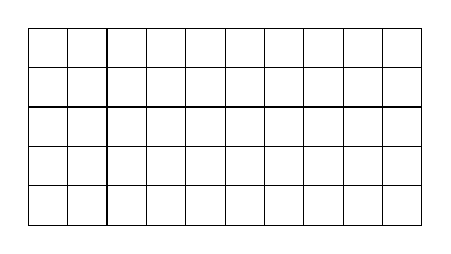
\begin{tikzpicture}
\draw[step=5mm, black] (0,0) grid (50mm,25mm);
\end{tikzpicture}

\end{center}
\begin{enumeratea}
 \item Colora con colori diversi i quadretti che servono per rappresentare i sei premi, un colore per ogni premio;
 \item quale parte del monte-premi è stata incassata da chi ha vinto il secondo premio?
	Esprimi questa parte con una frazione;
 \item Marco ha vinto il sesto premio: quanto ha vinto?
\end{enumeratea}
\end{esercizio}

\begin{esercizio}[\Ast]
 \label{ese:3.3}
La figura seguente è composta da~$11$ quadratini, alcuni bianchi altri grigi.
\begin{center}
 % (c) 2012 Dimitrios Vrettos - d.vrettos@gmail.com
% Esercizio 3.3
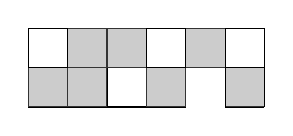
\begin{tikzpicture}
  \begin{scope}[step=5mm, black]
    \draw (0,0) grid (20mm,10mm);
    \draw (20mm,5mm) grid (25mm,10mm);
    \draw (25mm,0) grid (30mm,10mm);
  \end{scope}
  \begin{scope}[gray, opacity=.4]
    \fill (0,0) rectangle (10mm,5mm);
    \fill (15mm,0) rectangle (20mm,5mm);
    \fill (25mm,0) rectangle (30mm,5mm);
    \fill (5mm,5mm) rectangle (15mm,10mm);
    \fill (20mm,5mm) rectangle (25mm,10mm);   
  \end{scope}
  \draw (25mm,0)--(25mm,5mm);
\end{tikzpicture}

\end{center}
Quale frazione rappresenta la parte grigia rispetto all'intera figura? Quale frazione la parte bianca?
\end{esercizio}
\pagebreak
\begin{esercizio}
 \label{ese:3.4}
 Di ciascuna figura colora la parte indicata dalla frazione.
\begin{center}
 % (c) 2012 Dimitrios Vrettos - d.vrettos@gmail.com
% Esercizio 3.4

\begin{tikzpicture}

\draw  (0,0) circle(.8cm);
\draw (1.8cm,-.8cm) rectangle (4.1cm,.8cm);
\node [star, star point height=.5cm, minimum size=1.8cm, rotate=45, draw] at (5.9cm,0) {};

\node (cercio) at (0,1.5cm) {$\displaystyle\frac{3}{5}$};
\node (rettangolo) at (2.95cm,1.5cm) {$\displaystyle\frac{2}{3}$};
\node (cercio) at (5.9cm,1.5cm) {$\displaystyle\frac{1}{2}$};
\end{tikzpicture}

\end{center}
\end{esercizio}

\begin{esercizio}
\label{ese:3.5}
 Indica se le frazioni sono proprie (P), improprie (I) o apparenti (A).
 \begin{multicols}{3}
 \TabPositions{0.6cm}
 \begin{enumeratea}
 \item $\dfrac{3}{4}$ \tab\quad\boxP\quad\boxI\quad\boxA\vspace{1.1ex}
 \item $\dfrac{8}{3}$ \tab\quad\boxP\quad\boxI\quad\boxA
 \item $\dfrac{12}{3}$ \tab\quad\boxP\quad\boxI\quad\boxA\vspace{1.1ex}
 \item $\dfrac{5}{2}$ \tab\quad\boxP\quad\boxI\quad\boxA
 \item $\dfrac{5}{3}$ \tab\quad\boxP\quad\boxI\quad\boxA\vspace{1.1ex}
 \item $\dfrac{3}{2}$ \tab\quad\boxP\quad\boxI\quad\boxA
 \end{enumeratea}
 \end{multicols}
\end{esercizio}

\begin{esercizio}
\label{ese:3.6}
Trova le frazioni equivalenti completando.
 \begin{multicols}{4}
 \begin{enumeratea}
 	\item $\dfrac{3}{4}=\dfrac{\ldots}{12}$;
 	\item $\dfrac{12}{16}=\dfrac{3}{\ldots}$;
 	\item $\dfrac{5}{2}=\dfrac{\ldots}{10}$;
 	\item $\dfrac{21}{35}=\dfrac{\ldots}{5}$.
 \end{enumeratea}
 \end{multicols}
\end{esercizio}

\begin{esercizio}
\label{ese:3.7}
Sottolinea le frazioni equivalenti a~$\dfrac{3}{5}$ tra le seguenti.
\[\frac{6}{10};\qquad\frac{25}{100};\qquad\frac{12}{10};\qquad\frac{5}{25}.\]
\end{esercizio}

\begin{esercizio}
\label{ese:3.8}
Completa le seguenti uguaglianze.
\begin{multicols}{4}
\begin{enumeratea}
\item $\displaystyle{\frac{3}{5}=\frac{\ldots}{10}}$;
\item $\displaystyle{\frac{75}{10}=\frac{\ldots}{100}}$;
\item $\displaystyle{\frac{7}{\ldots}=\frac{1}{2}}$;
\item $\displaystyle{3=\frac{24}{\ldots}}$.
\end{enumeratea}
\end{multicols}
\end{esercizio}

\begin{esercizio}
 \label{ese:3.9}
 Indica almeno tre frazioni equivalenti a ciascuna delle seguenti.
 \begin{multicols}{6}
 \begin{enumeratea}
 	\item $\dfrac{5}{6}$;
 	\item $\dfrac{3}{5}$;
 	\item $\dfrac{12}{60}$;
 	\item $\dfrac{2}{3}$;
 	\item $\dfrac{1}{2}$;
 	\item $\dfrac{5}{2}$.
 \end{enumeratea}
 \end{multicols}
\end{esercizio}

\begin{esercizio}
 \label{ese:3.10}
Nella figura che segue il quadratino colorato rappresenta~$1/4$ del quadrato grande; costruisci una figura
che rappresenti~$8/4$ del quadrato grande accostando opportunamente altri quadrati uguali.
 \begin{center}
 % (c) 2012 Dimitrios Vrettos - d.vrettos@gmail.com
% Quadrato 1/4
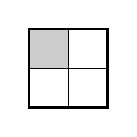
\begin{tikzpicture}
  \begin{scope}[scale=1,every node/.style={minimum size=5mm}]
    \draw[step=5mm, black] (0,0) grid (1,1);
    \fill[gray, opacity=.4] (0,.5) rectangle (.5,1);
    \draw[black,thick] (0,0) rectangle (1,1);
  \end{scope} 
\end{tikzpicture}

 \end{center}
\end{esercizio}

\begin{esercizio}
 \label{ese:3.11}
Riduci ai minimi termini le seguenti frazioni.
 \begin{multicols}{6}
 \begin{enumeratea}
 \item $\dfrac{4}{6}$;\vspace{1.1ex}
 \item $\dfrac{8}{2}$;\vspace{1.1ex}
 \item $\dfrac{2}{10}$;
 \item $\dfrac{18}{16}$;\vspace{1.1ex}
 \item $\dfrac{3}{12}$;\vspace{1.1ex}
 \item $\dfrac{6}{20}$;
 \item $\dfrac{80}{100}$;\vspace{1.1ex}
 \item $\dfrac{8}{12}$;\vspace{1.1ex}
 \item $\dfrac{9}{6}$;
 \item $\dfrac{10}{15}$;\vspace{1.1ex}
 \item $\dfrac{14}{49}$;\vspace{1.1ex}
 \item $\dfrac{15}{21}$;
 \item $\dfrac{16}{6}$;\vspace{1.1ex}
 \item $\dfrac{18}{15}$;\vspace{1.1ex}
 \item $\dfrac{20}{12}$;
 \item $\dfrac{21}{9}$;\vspace{1.1ex}
 \item $\dfrac{24}{30}$;\vspace{1.1ex}
 \item $\dfrac{25}{15}$.
 \end{enumeratea}
 \end{multicols}
\end{esercizio}

\begin{esercizio}
 \label{ese:3.12}
Riduci ai minimi termini le seguenti frazioni.
 \begin{multicols}{6}
 \begin{enumeratea}
 \item $\dfrac{27}{21}$;\vspace{1.1ex}
 \item $\dfrac{28}{14}$;\vspace{1.1ex}
 \item $\dfrac{30}{16}$;
 \item $\dfrac{32}{24}$;\vspace{1.1ex}
 \item $\dfrac{35}{10}$;\vspace{1.1ex}
 \item $\dfrac{36}{81}$;
 \item $\dfrac{40}{6}$;\vspace{1.1ex}
 \item $\dfrac{42}{21}$;\vspace{1.1ex}
 \item $\dfrac{45}{27}$;
 \item $\dfrac{48}{60}$;\vspace{1.1ex}
 \item $\dfrac{12}{30}$;\vspace{1.1ex}
 \item $\dfrac{135}{77}$.
% \item $\dfrac{121}{22}$;\vspace{1.1ex}
% \item $\dfrac{87}{99}$;\vspace{1.1ex}
% \item $\dfrac{15}{360}$;
% \item $\dfrac{110}{30}$;\vspace{1.1ex}
% \item $\dfrac{240}{75}$;\vspace{1.1ex}
% \item $\dfrac{140}{294}$.
 \end{enumeratea}
 \end{multicols}
\end{esercizio}

\begin{figure}[t]
 \begin{minipage}[b]{.45\textwidth}
 \centering% (c) 2012 Dimitrios Vrettos - d.vrettos@gmail.com
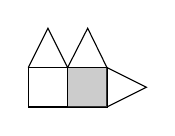
\begin{tikzpicture}
\draw (0,0) rectangle  (10mm,5mm);
\draw (0,5mm) -- (2.5mm,10mm)--(5mm,5mm)--(7.55mm,10mm)--(10mm,5mm);
\draw (10mm,5mm) -- (15mm,2.5mm)--(10mm,0);
\draw (5mm,0) -- (5mm,5mm);

\fill[gray, opacity=.4](5mm,0) rectangle  (10mm,5mm);
\end{tikzpicture}

 \caption{Esercizio~\ref{ese:3.13}}\label{fig:3.4}
 \end{minipage}\hfil
\begin{minipage}[b]{.45\textwidth}
 \centering% (c) 2012 Dimitrios Vrettos - d.vrettos@gmail.com
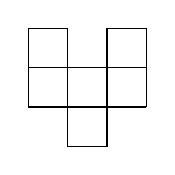
\begin{tikzpicture}
\draw[step=5mm] (0,0) grid  (15mm,5mm);
\draw (0,5mm) rectangle  (5mm,10mm);
\draw (10mm,5mm) rectangle  (15mm,10mm);
\draw (5mm,0) rectangle  (10mm,-5mm);
\end{tikzpicture}

 \caption{Esercizio~\ref{ese:3.14}}\label{fig:3.5}
 \end{minipage}
\end{figure}

\begin{esercizio}
 \label{ese:3.13}
Si può dire che la parte colorata in grigio della figura \ref{fig:3.4} corrisponde a~$\frac{1}{5}$ della figura stessa?
\end{esercizio}

\begin{esercizio}
 \label{ese:3.14}
Costruisci una figura che corrisponde a~$\frac{11}{6}$ della figura \ref{fig:3.5}.
\end{esercizio}

\begin{esercizio}
 \label{ese:3.15}
Per quali dei seguenti disegni la parte colorata in grigio rappresenta sempre la frazione~$\dfrac{3}{4}$
del quadrato bianco?
 \begin{center}
 % (c) 2012 Dimitrios Vrettos - d.vrettos@gmail.com
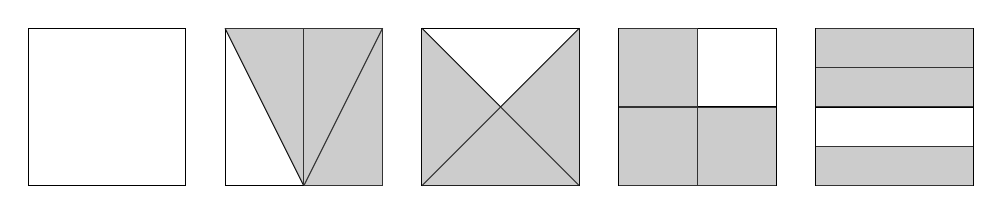
\begin{tikzpicture}
  \begin{scope}[x=25mm,y=5mm]
    % Costruzione dei 5 quadrati
    \foreach \x in {0,1,...,4}
      \node[draw, minimum size=20mm](quad) at(\x,0) {};
    %  Nomi
%     \foreach \c [count=\x from 0] in {$A$,$B$,$C$,$D$,$E$} 
%       \node[below=13mm] at (\x,0) {\c};
    %  quadrato B
    \draw(15mm,2)--(1,-2);
    \draw(1,-2)--(35mm,2);
    \draw(1,-2)--(1,2);
    \begin{scope}[fill=gray, fill opacity=.4]
      \fill (15mm,2)--(1,2)--(1,-2);
      \fill (1,-2) rectangle (35mm,2);
    \end{scope}
    % quadrato C
    \draw(40mm,2)--(60mm,-2);
    \draw (40mm,-2) -- (60mm,2);
    \begin{scope}[fill=gray, fill opacity=.4]
      \fill (40mm,2)--(60mm,-2)--(40mm,-2);
      \fill (60mm,2)--(60mm,-2)--(2,0);
    \end{scope}
    % quadrato D
    \draw (65mm,0) -- (85mm,0);
    \draw (3,-2) -- (3,2);
    \begin{scope}[fill=gray, fill opacity=.4]
      \fill (65mm,-2) rectangle (3,2);
      \fill (3,-2) rectangle (85mm,0);
    \end{scope}
    % quadrato E
    \foreach \y in {-1,0,1}
      \draw (90mm,\y) -- (110mm,\y);
    \begin{scope}[fill=gray, fill opacity=.4]
      \fill (90mm,2) rectangle (110mm,0);
      \fill (90mm,-2) rectangle (110mm,-1);
    \end{scope}
  \end{scope}
\end{tikzpicture}

 \end{center}
\end{esercizio}

\begin{figure}[t]
 \begin{minipage}[b]{.20\textwidth}
 \centering% (c) 2012 Dimitrios Vrettos - d.vrettos@gmail.com
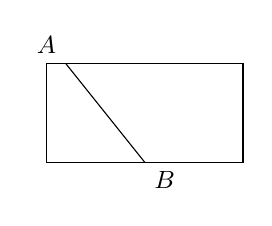
\begin{tikzpicture}[x=5mm,y=5mm,font=\small]
  \draw (0,0) rectangle (5,2.5);
  \draw (.5,2.5)node [above left] () {$A$} -- (2.5,0)node [below right] () {$B$};
\end{tikzpicture}

 \caption{\ref{ese:3.16}}\label{fig:3.6}
 \end{minipage}\hfil
 \begin{minipage}[b]{.20\textwidth}
 \centering % (c) 2012 Dimitrios Vrettos - d.vrettos@gmail.com
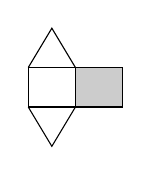
\begin{tikzpicture}[x=6mm,y=5mm]
\fill[gray, opacity=.4](1,0) rectangle (2,1);
\foreach \x in {0,1}
\draw (\x,0) rectangle  (\x+1,1);
\foreach \x in {0}
\foreach \y in {1}{
\draw (\x,\y) -- (\x+.5,\y+1)--(\x+1,\y);
\draw(\x,\y-1)--(\x+.5,-\y)--(\x+1,\y-1);}
\end{tikzpicture}

 \caption{\ref{ese:3.17}}\label{fig:3.7}
 \end{minipage}\hfil
 \begin{minipage}[b]{.20\textwidth}
 \centering% (c) 2012 Dimitrios Vrettos - d.vrettos@gmail.com
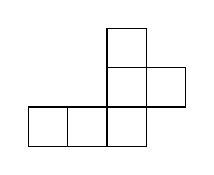
\begin{tikzpicture}[x=5mm,y=5mm]
\foreach \x in {0,1,2}
\draw (\x,0) rectangle (\x+1,1);
\foreach \y in {1,2}
\draw (2,\y) rectangle (3,\y+1);
\draw(3,1) rectangle (4,2);
\end{tikzpicture}

 \caption{\ref{ese:3.18}}\label{fig:3.8}
 \end{minipage}\hfil
 \begin{minipage}[b]{.23\textwidth}
 \centering% (c) 2012 Dimitrios Vrettos - d.vrettos@gmail.com
\begin{tikzpicture}[x=5mm,y=5mm]
\draw (0,0) rectangle (3,3);
\end{tikzpicture}

 \caption{\ref{ese:3.19}}\label{fig:3.9}
 \end{minipage}\hfil
\end{figure}

\begin{esercizio}
\label{ese:3.16}
Relativamente alla figura~\ref{fig:3.6}, quale proposizione è vera?

\begin{enumeratea}
\item Il segmento~$AB$ la divide in due parti uguali;
\item il segmento~$AB$ la divide in due quadrilateri.
\end{enumeratea}
\end{esercizio}

 \begin{esercizio}
 \label{ese:3.17}
La parte in grigio rappresenta~$1/4$ della figura~\ref{fig:3.7}?
\end{esercizio}

\begin{esercizio}
\label{ese:3.18}
 Costruisci una figura che sia gli~$11/6$ della figura~\ref{fig:3.8}.
\end{esercizio}

\begin{esercizio}
\label{ese:3.19}
Colora i~$3/4$ della figura~\ref{fig:3.9}.
\end{esercizio}

\begin{esercizio}
 \label{ese:3.20}
Il segmento nel disegno rappresenta i~$3/5$ dell'intero.
 \begin{center}
 % (c) 2012 Dimitrios Vrettos - d.vrettos@gmail.com
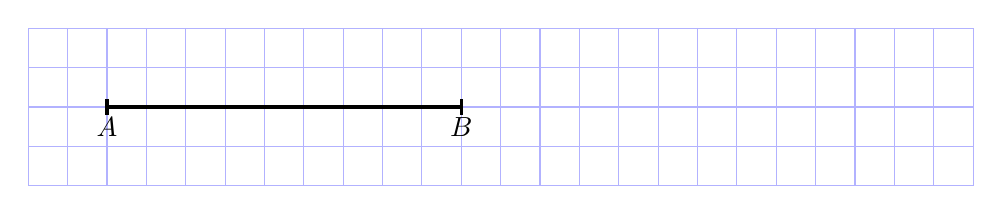
\begin{tikzpicture}
\draw[step=5mm, blue, opacity=.3](0,0) grid (120mm,20mm);
\draw[very thick](10mm,10mm) node [below] {$A$} --(55mm,10mm) node [below] {$B$};
\draw[very thick](10mm,9mm) -- (10mm,11mm);
\draw[very thick](55mm,9mm) -- (55mm,11mm);
\end{tikzpicture}

 \end{center}
Ti basta questa informazione per costruire l'intero? Come procederesti?
\end{esercizio}

\begin{esercizio}
 \label{ese:3.21}
Disegna un segmento come grandezza unitaria e dimostra che la frazione~$3/5$ è equivalente a~$6/10$ ma non a~$9/25$.
% \begin{center}
% % (c) 2012 Dimitrios Vrettos - d.vrettos@gmail.com

\begin{tikzpicture}
\draw[step=5mm, blue, opacity=.3](0,0) grid (140mm,20mm);
\end{tikzpicture}

% \end{center}
\end{esercizio}

%\begin{esercizio}eliminato da Antonio
% \label{ese:3.16}
%Usando una grandezza unitaria arbitraria, stabilisci quale delle seguenti frazioni
%rappresenta l'intero e quale un suo multiplo:
%\[\dfrac{2}{4}\text{,}\qquad\dfrac{6}{3}\text{,}\qquad\dfrac{5}{5}\text{,}\qquad\dfrac{8}{4}\text{,}\qquad
%\dfrac{9}{4}.\]
%\end{esercizio}

%%%%%%%%%%%%%%%%%%%%%%%%%%%%%%%%%%%%%%%%%%%%
%~3.3 Dalle frazioni ai numeri razionali %
%%%%%%%%%%%%%%%%%%%%%%%%%%%%%%%%%%%%%%%%%%%%
\subsubsection*{3.3 - Dalle frazioni ai numeri razionali}

%\begin{esercizio}
% \label{ese:3.17}eliminato da Antonio
%Raggruppa le seguenti frazioni in insiemi di frazioni equivalenti.
%Etichetta l'insieme con un numero razionale, prendendo per ogni gruppo la frazione ridotta ai minimi termini.
%
%\[\frac{1}{3};\,\frac{2}{4};\,-\frac{5}{2};\,\frac{6}{-14};\,\frac{-12}{4};\,\frac{3}{6};\,\frac{-3}{-9};\,
%\frac{10}{-4};\,\frac{10}{20};\,\frac{-18}{42};\,\frac{5}{15};\,-\frac{9}{21};\,-\frac{15}{6};\,\frac{4}{12}.\]
%\end{esercizio}

\begin{esercizio}
 \label{ese:3.22}
 Riscrivi le seguenti frazioni improprie come somma di un numero naturale e una frazione propria.
\[\frac{10}{3};\,\frac{17}{9};\,\frac{11}{2};\,\frac{25}{3};\,\frac{17}{10};\,\frac{15}{6}.\]
\end{esercizio}

\subsubsection*{3.4 - La scrittura dei numeri razionali}

\begin{esercizio}
 \label{ese:3.23}
 Senza eseguire le divisioni indica quali di queste frazioni possono essere scritte come numero decimale
finito (DF), quali come numero decimale periodico (DP)
e quali come numero intero (I):
 \begin{multicols}{2}
 \TabPositions{1cm}
 \begin{enumeratea}
% 	\spazielenx
 \item $-\dfrac{3}{2}$ \tab\qquad\boxDF\qquad\boxDP\quad\:\:\boxI\vspace{1.1ex}
 \item $-\dfrac{6}{5}$ \tab\qquad\boxDF\qquad\boxDP\quad\:\:\boxI\vspace{1.1ex}
 \item $\dfrac{2}{25}$ \tab\qquad\boxDF\qquad\boxDP\quad\:\:\boxI\vspace{1.1ex}
 \item $\dfrac{5}{8}$ \tab\qquad\boxDF\qquad\boxDP\quad\:\:\boxI
 \item $\dfrac{5}{6}$ \tab\qquad\boxDF\qquad\boxDP\quad\:\:\boxI\vspace{1.1ex}
 \item $-\dfrac{5}{12}$ \tab\qquad\boxDF\qquad\boxDP\quad\:\:\boxI\vspace{1.1ex}
 \item $\dfrac{12}{6}$ \tab\qquad\boxDF\qquad\boxDP\quad\:\:\boxI\vspace{1.1ex}
 \item $\dfrac{5}{10}$ \tab\qquad\boxDF\qquad\boxDP\quad\:\:\boxI
 \end{enumeratea}
 \end{multicols}
\end{esercizio}

\begin{esercizio}[\Ast]
\label{ese:3.24}
Trasforma le seguenti frazioni in numeri decimali.
\begin{multicols}{5}
\begin{enumeratea}
\spazielenx
\item $\dfrac{13}{2}$;
\item $\dfrac{11}{3}$;
\item $\dfrac{3}{5}$;
\item $\dfrac{15}{6}$;
\item $\dfrac{17}{7}$;
\item $\dfrac{15}{8}$;
\item $\dfrac{12}{9}$;
\item $\dfrac{127}{10}$;
\item $\dfrac{122}{11}$;
\item $\dfrac{13}{12}$;
\item $\dfrac{35}{121}$;
\item $\dfrac{121}{35}$;
\item $\dfrac{12}{10}$;
\item $\dfrac{127}{100}$;
\item $\dfrac{122}{\np{1100}}$;
\item $\dfrac{13}{100}$;
\item $\dfrac{35}{\np{1000}}$;
\item $\dfrac{121}{\np{10000}}$;
\item $\dfrac{12}{5}$;
\item $\dfrac{13}{7}$;
\item $\dfrac{15}{4}$;
\item $\dfrac{5}{8}$;
\item $\dfrac{32}{9}$;
\item $\dfrac{21}{20}$;
\item $\dfrac{37}{18}$;
%\item $\dfrac{2}{21}$.
\end{enumeratea}
\end{multicols}
\end{esercizio}
\pagebreak
\begin{esercizio}
\label{ese:3.25}
Trasforma le seguenti frazioni in numeri decimali.
\begin{multicols}{4}
\begin{enumeratea}
\spazielenx
\item $\dfrac{4}{12}$;
\item $\dfrac{20}{15}$;
\item $\dfrac{135}{1}$;
\item $\dfrac{28}{49}$;
\item $\dfrac{45}{9}$;
\item $\dfrac{80}{5}$;
\item $\dfrac{8}{50}$;
\item $\dfrac{36}{1080}$;
\item $\dfrac{55}{6875}$;
\item $\dfrac{54}{648}$;
\item $\dfrac{25}{\np{0,0000002}}$;
\item $\dfrac{28}{\np{0,00000049}}$;
\item $\dfrac{40}{\np{0,000002}}$;
\item $\dfrac{45}{\np{0,00009}}$;
\item $\dfrac{0,008}{10\times 10^{-3}}$;
\item $\dfrac{800}{5\times 10^{4}}$;
\item $\dfrac{8\times 10^{2}}{\np{50000}}$;
\item $\dfrac{12^{4}}{3^{3} \times 2^{6}}$;
\item $\dfrac{8\times 10^{-3}}{\np{0,005}}$;
\item $\dfrac{2^{3}\times \np{1000}}{500}$;
\item $\dfrac{2^{8}\times 5^{8}}{10^{8}}$;
\item $\dfrac{3^{18}}{9^{9}}$.
\end{enumeratea}
\end{multicols}
\end{esercizio}

\begin{esercizio}[\Ast]
\label{ese:3.26}
Trasforma in frazioni i seguenti numeri decimali.
\begin{multicols}{4}
\begin{enumeratea}
 \item $\np{12,5}$;
 \item $\np{4,2}$;
 \item $\np{6,25}$;
 \item $\np{3,75}$;
 \item $\np{0,1}$;
 \item $\np{2,5}$;
 \item $\np{100,100}$;
 \item $\np{0,12}$;
 \item $\np{1,1030}$;
 \item $\np{0,00100}$;
 \item $\np{100,0010}$;
 \item $\np{0,0001}$;
 \item $\np{1,25}$;
 \item $\np{0,08}$;
 \item $\np{1,002}$;
 \item $\np{15,675}$;
 \item $\np{1,7}$;
 \item $\np{1,46}$;
 \item $\np{0,13}$;
 \item $\np{0,149}$;
 \item $\np{5,015}$;
 \item $\np{3,21}$;
 \item $\np{2,3}$;
 \item $\np{1,086}$.
\end{enumeratea}
\end{multicols}
\end{esercizio}


\begin{esercizio}
 \label{ese:3.27}
Completa la tabella.

 \begin{tabular*}{.9\textwidth}{@{\extracolsep{\fill}}*{6}{lccccc}}
 \toprule
 &\multicolumn{2}{c}{Parte}& & &\\
 Numero decimale & intera & decimale & Periodo & Antiperiodo & Frazione\\
 \midrule
~$1,752\,1$& & &	& &\\
~$3,\overline{75}$& & &	& &\\
~$12,1\overline{24}$& & &	& &\\
~$1,0\overline{5}~$& & &	& &\\
~$0,13\overline{57}~$& & &	& &\\
 \bottomrule
 \end{tabular*}
\end{esercizio}

%\clearpage
\begin{esercizio}[\Ast]
\label{ese:3.28}
 Trasforma i seguenti numeri decimali in frazioni.
\begin{multicols}{4}
\begin{enumeratea}
\item $\np{-1,25}$;
\item $\np{0,03}$;
\item $\np{-2,}\overline{1}$;
\item $\np{0,}\overline{13}$;
\item $\np{5,080}$;
\item $\np{3,7}\overline{52}$;
\item $\np{-0,38}$;
\item $\np{11,}\overline{175}$;
\item $\np{0,01}\overline{0\,2}$
\item $\np{0,12}\overline{3\,45}$;
\item $\np{100,}\overline{100}$;
\item $\np{100,}\overline{001}$;
\item $\np{0,08}$;
\item $\np{0,2}$;
\item $\np{0,1}$;
\item $\np{0,03}$;
\item $\np{23,}\overline{5}$;
\item $\np{22,}\overline{32}$;
\item $\np{0,25}$;
\item $\np{31,}\overline{02}$;
\item $\np{0,}\overline{21}$;
\item $\np{2,3}\overline{4}$;
\item $\np{3,21}\overline{8}$;
\item $\np{0,03}\overline{4}$.
\end{enumeratea}
\end{multicols}
\end{esercizio}
\pagebreak
\begin{esercizio}
\label{ese:3.29}
 Scrivi delle frazioni equivalenti ai seguenti numeri decimali.
\begin{multicols}{4}
\begin{enumeratea}
\item $\np{0,00355}$;
\item $\np{3,7}$;
\item $\np{7,84}$;
\item $\np{0,004}\cdot 10^{5}$;
\item $\np{0,001}^{3}$;
\item $\np{7,42}$;
\item $\np{-0,00}\overline{6}$;
\item $\np{3}\cdot 10^{-4}$.
\end{enumeratea}
\end{multicols}
\end{esercizio}

\begin{esercizio}
\label{ese:3.30}
Scrivi la frazione generatrice di~$\np{12,3}\overline{45}$. Qual è la~614-esima cifra decimale del numero?
\end{esercizio}

\begin{esercizio}
\label{ese:3.31}
Calcola~$\np{0,}\overline{9}-\np{3,}\overline{9}$. Cosa osservi?
\end{esercizio}

\begin{esercizio}
\label{ese:3.32}
Verifica le seguenti uguaglianze trovando la frazione generatrice.
\[\frac{\np{1,}\overline{7}}{\np{1,}\overline{3}}=\np{1,}\overline{3};\qquad%
\frac{\np{2,}\overline{7}}{\np{1,}\overline{6}}=\np{1,}\overline{6};\qquad%
\frac{\np{1,}\overline{16}}{\np{2,}\overline{3}}=\np{0,5};\qquad%
\frac{\np{2,}\overline{3}}{\np{1,}\overline{6}}=\np{1,4}.\]
\end{esercizio}

\subsubsection*{3.5 - I numeri razionali e la retta}

\begin{esercizio}
 \label{ese:3.33}
Rappresenta su una retta orientata, dopo aver scelto una opportuna unità di misura,
i seguenti gruppi di numeri razionali, ciascun gruppo su una retta.
 \begin{enumeratea}
\spazielenx
 \item $\displaystyle{\frac{2}{3}\text{,}\quad-\frac{3}{4}\text{,}\quad\frac{5}{2}\text{,}\quad-\frac{7}{12}\text{,}\quad\frac{3}{2}\text{,}\quad%
-\frac{11}{6}\text{,}\quad\frac{9}{4}}$;
 \item $\displaystyle{\frac{0}{4}\text{,}\quad\frac{5}{4}\text{,}\quad\frac{9}{4}\text{,}\quad\frac{1}{2}\text{,}\quad\frac{19}{8}\text{,}\quad\frac{3}{2}%
\text{,}\quad\frac{7}{4}\text{,}\quad\frac{4}{2}}$;
 \item $\displaystyle{\frac{10}{3}\text{,}\quad\frac{5}{3}\text{,}\quad~2\text{,}\quad\frac{0}{3}\text{,}\quad\frac{4}{3}\text{,}\quad\frac{2}{3}%
\text{,}\quad\frac{5}{6}\text{,}\quad\frac{13}{6}}$;
 \item $\displaystyle{\frac{1}{2}\text{,}\quad\frac{3}{4}\text{,}\quad-\frac{5}{4}\text{,}\quad-\frac{1}{2}\text{,}\quad\frac{7}{8}\text{,}%
\quad-\frac{5}{16}}$;
\item $\displaystyle{\frac{8}{5}\text{,}\quad\frac{1}{2}\text{,}\quad\frac{3}{10}\text{,}\quad-\frac{7}{4}\text{,}\quad-\frac{3}{5}%
\text{,}\quad-\frac{11}{10}}$.
 \end{enumeratea}
\end{esercizio}

\begin{esercizio}
 \label{ese:3.34}
 Scrivi i numeri razionali rappresentati dai punti segnati sulla retta nella figura.
\begin{center}
% (c) 2012 Dimitrios Vrettos - d.vrettos@gmail.com
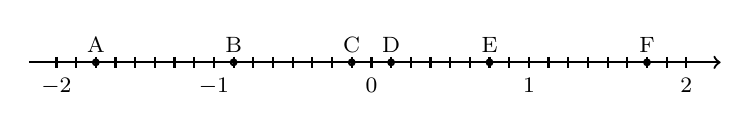
\begin{tikzpicture}
\begin{scope}[thick,font=\footnotesize]
\draw[->] (-10pt,0) -- (240pt,0);
  \foreach \x/\xtext in {%
      0/-2,.25/,.5/,.75/,
1/,1.25/,1.5/,1.75/,2/-1,2.25/,2.5/,2.75/,3/,%
      3.25/,3.5/,3.75/,4/0,4.25/,4.5/,4.75/,%
      5/,5.25/,5.5/,5.75/,6/1,6.25/,6.5/,6.75/,7/,7.25/,7.5/,7.75/,8/2}
    \draw[shift={(\x,0)}] (0pt,2pt) -- (0pt,-2pt) node[below] {$\xtext$};
\foreach \y/\ytext in {.5/$A$,2.25/$B$,3.75/$C$,4.25/$D$,5.5/$E$,7.5/$F$}
	 \draw[shift={(\y,0)}] (0pt,2pt) -- (0pt,-2pt) node[above=2pt] {$\ytext$};
\draw (.5,0) circle (1pt);
\draw (2.25,0) circle (1pt);
\draw (3.75,0) circle (1pt);
\draw (4.25,0) circle (1pt);
\draw (5.5,0) circle (1pt);
\draw (7.5,0) circle (1pt);
\end{scope}
\end{tikzpicture}

\end{center}
$ A=\ldots $,\quad $ B=\ldots $,\quad $ C=\ldots $,\quad $ D=\ldots $,\quad $ E=\ldots $,\quad $ F=\ldots $.

\end{esercizio}

\begin{esercizio}
 \label{ese:3.35}
Rappresenta su una opportuna retta numerica le seguenti frazioni.
\[\frac{3}{4};\quad\frac{3}{8};\quad\frac{1}{3};\quad\frac{5}{4};\quad\frac{2}{5};\quad\frac{6}{3};\quad\frac{5}{6};\quad%
\frac{12}{4};\quad\frac{19}{8};\quad\frac{16}{5}.\]
\end{esercizio}

\begin{esercizio}
 \label{ese:3.36}
Disegna su una retta orientata i seguenti numeri decimali, ciascun gruppo su una retta diversa.
\begin{enumeratea}
 \item $\np{0,6}$,$\qquad\np{2,3}$,$\qquad\np{-1,2}$,$\qquad\np{-0,06}$;
 \item $\np{+1,4}$,$\qquad\np{-0,3}$,$\qquad\np{-1,5}$,$\qquad\np{0,2}$;
 \item $\np{-0,8}$,$\qquad\np{-1,6}$,$\qquad\np{+4,91}$,$\qquad\np{-1,17}$;
 \item $\np{1,55}$,$\qquad\np{2,01}$,$\qquad\np{-3,0}$,$\qquad\np{-2,10}$.
\end{enumeratea}
\end{esercizio}
\pagebreak
\subsubsection*{3.6 - Confronto tra numeri razionali}

\begin{esercizio}
 \label{ese:3.37}
Inserisci tra le seguenti coppie di numeri razionali i simboli di maggiore~($>$), minore~($<$) o uguale~($=$).
\begin{multicols}{3}
\begin{enumeratea}
\spazielenx
 \item $\dfrac{4}{5}\,\ldots\,\dfrac{5}{7}$;
 \item $-\dfrac{9}{5}\,\ldots\,-\dfrac{8}{3}$;
 \item $-1\,\ldots\,\dfrac{1}{12}$;
 \item $\dfrac{2}{7}\,\ldots\,\dfrac{6}{21}$;
 \item $-\dfrac{1}{2}\,\ldots\,-\dfrac{3}{4}$;
 \item $\dfrac{3}{5}\,\ldots\,\dfrac{6}{9}$.
\end{enumeratea}
\end{multicols}
\end{esercizio}

\begin{esercizio}
 \label{ese:3.38}
Riscrivi in ordine crescente (dalla più piccola alla più grande) le seguenti frazioni.
\begin{enumeratea}
\item $\dfrac{2}{3}\text{,}\qquad\dfrac{3}{4}\text{,}\qquad\dfrac{5}{8}\text{,}\qquad\dfrac{3}{5}\text{,}\qquad\dfrac{7}{12}$;
\item $-\dfrac{2}{3}\text{,}\qquad-\dfrac{3}{4}\text{,}\qquad-\dfrac{5}{6}\text{,}\qquad-\dfrac{1}{2}\text{,}\qquad-\dfrac{2}{5}$;
\item $-\dfrac{2}{3}\text{,}\qquad\dfrac{3}{4}\text{,}\qquad-\dfrac{5}{6}\text{,}\qquad\dfrac{1}{2}\text{,}\qquad-1\text{,}\qquad-\dfrac{2}{5}\text{,}\qquad0.$
\item $-\dfrac{3}{2}\text{,}\qquad\dfrac{4}{3}\text{,}\qquad-\dfrac{6}{5}\text{,}\qquad\dfrac{2}{5}\text{,}\qquad-1\text{,}\qquad\dfrac{5}{2}\text{,}\qquad0$
\item $\dfrac{3}{4}\text{,}\qquad\dfrac{4}{3}\text{,}\qquad\dfrac{11}{12}\text{,}\qquad\dfrac{5}{3}\text{,}\qquad\dfrac{2}{3}\text{,}\qquad\dfrac{2}{7}\text{,}\qquad\dfrac{3}{2}$.
\end{enumeratea}
\end{esercizio}

\begin{esercizio}
 \label{ese:3.39}
Ordina dal più piccolo al più grande i seguenti valori.
\begin{enumeratea}
\item $\np{10,011}$,$\qquad\np{10,110}$,$\qquad\np{11,001}$,$\qquad\np{11,100}$;
\item $\np{10,01}$,$\qquad\np{11,11}$,$\qquad\np{10,101}$,$\qquad\np{10,001}$;
\item $\np{0,101}$,$\qquad\np{0,011}$,$\qquad\np{0,110}$,$\qquad\np{0,0101}$;
\item $\np{1,0101}$,$\qquad\np{1,1001}$,$\qquad\np{1,0011}$,$\qquad\np{1,0110}$.
\end{enumeratea}
\end{esercizio}

\begin{esercizio}
\label{ese:3.40}
Scrivi una frazione molto vicina a~$-\dfrac{2}{9}.$
\end{esercizio}

\begin{esercizio}
\label{ese:3.41}
Scrivi una frazione compresa tra:
\begin{multicols}{3}
\begin{enumeratea}
\item $\dfrac{3}{5}$ e~$\dfrac{7}{10}$;
\item $\dfrac{5}{3}$ e~$\dfrac{1}{7}$;
\item $\dfrac{1}{2}$ e~$\dfrac{2}{3}$.
\end{enumeratea}
\end{multicols}
\end{esercizio}

\begin{esercizio}
\label{ese:3.42}
Quali disuguaglianze sono vere?
\begin{multicols}{2}
\TabPositions{2.5cm}
\begin{enumeratea}
\spazielenx
 \item $-\dfrac{7}{6}<-\dfrac{6}{7}$;\tab\boxV\qquad\boxF
 \item $-\dfrac{7}{6}>+\dfrac{6}{7}$;\tab\boxV\qquad\boxF
 \item $-\dfrac{7}{6}<+\dfrac{6}{7}$;\tab\boxV\qquad\boxF
 \item $+\dfrac{7}{6}<-\dfrac{6}{7}$;\tab\boxV\qquad\boxF
 \item $+\dfrac{7}{6}<+\dfrac{6}{7}$;\tab\boxV\qquad\boxF
 \item $+\dfrac{7}{6}>-\dfrac{6}{7}$.\tab\boxV\qquad\boxF
 \end{enumeratea}
\end{multicols}
\end{esercizio}

\begin{esercizio}
\label{ese:3.43}
Quale dei seguenti numeri è più vicino a~1?
\[\boxA\quad\np{0,10}\qquad\boxB\quad\np{0,99}\qquad\boxC\quad\np{0,01}\qquad\boxD\quad\np{0,90}\]
\end{esercizio}

 \begin{esercizio}
\label{ese:3.44}
Quale dei seguenti numeri è più vicino alla frazione~$\dfrac{1}{10}$?
\[\boxA\quad\np{0,01}\qquad\boxB\quad\np{0,90}\qquad\boxC\quad\np{1,01}\qquad\boxD\quad\np{0,19}\]
 \end{esercizio}
\pagebreak
\begin{esercizio}
\label{ese:3.45}
Scrivi due numeri compresi tra:
\begin{multicols}{3}
\begin{enumeratea}
 \item $\np{2,3}$ e $\np{3,4}$;
 \item $\np{3,4}$ e $\np{3,6}$;
 \item $\np{2,}\overline{3}$ e~$\np{2,}\overline{4}$;
 \item $\np{1,1}\overline{3}$ e~$\np{1,2}\overline{3}$;
 \item $\np{3,}\overline{4}$ e~$\np{3,}\overline{6}$;
 \item $\np{1,}\overline{35}$ e~$\np{1,}\overline{36}$.
\end{enumeratea}
\end{multicols}
\end{esercizio}

%\begin{esercizio}
% \label{ese:3.43}
%Rappresenta su una opportuna retta numerica le seguenti frazioni e poi riscrivile in ordine
%crescente:
%\[\frac{3}{4}\text{,~~}\frac{3}{8}\text{,~~}\frac{1}{3}\text{,~~}\frac{5}{4}\text{,~~}\frac{2}{5}\text{,~~}\frac{6}{3}\text{,~~}\frac{5}{6}\text{,~~}\frac{12}{4}\text{,~~}\frac{19}{8}\text{,~~}\frac{16}{5}.\]
%\end{esercizio}

%%%%%%%%%%%%%%%%%%%%%%%%%%%%%%%%%%%%%%%%%%%%%%%%%%%%%%%%%%%
\subsubsection*{3.7 - Le operazioni con i numeri razionali}


\begin{esercizio}[\Ast]
 \label{ese:3.46}
Calcola le seguenti somme algebriche tra frazioni.
\begin{multicols}{4}
\begin{enumeratea}
\spazielenx
\item $\dfrac{1}{2} + \dfrac{3}{2}$;
\item $\dfrac{7}{11} + \dfrac{4}{11}$;
\item $\dfrac{3}{2} - \dfrac{5}{2}$;
\item $\dfrac{8}{18} + \dfrac{5}{9}$;
\item $\dfrac{6}{5} + 0$;
\item $-\dfrac{3}{2}+\dfrac{4}{3}$;
\item $-\dfrac{2}{3}+\dfrac{3}{4}$;
\item $\dfrac{4}{3}-\dfrac{6}{5}$;
\item $\dfrac{2}{5}+\dfrac{5}{8}$;
\item $\dfrac{5}{8}+\dfrac{5}{6}$;
\item $\dfrac{5}{6}-\dfrac{5}{12}$;
\item $1-\dfrac{3}{2}$;
\item $\dfrac{11}{5}+5$;
\item $\dfrac{7}{3}-\dfrac{6}{4}$;
\item $3-\dfrac{2}{3}$;
\item $\dfrac{1}{5}-1$;
\item $4+\dfrac{3}{2}-\dfrac{3}{4}$;
\item $\dfrac{4}{3}+3-\dfrac{1}{2}$;
\item $\dfrac{3}{4}+\dfrac{1}{4}-\dfrac{5}{4}$;
\item $1-\dfrac{1}{2}+\dfrac{1}{3}-\dfrac{1}{4}$.
\end{enumeratea}
\end{multicols}
\end{esercizio}

\begin{esercizio}
 \label{ese:3.47}
Calcola le seguenti somme algebriche fra numeri razionali.
\begin{multicols}{3}
\begin{enumeratea}
\spazielenx
\item $\np{1,}\overline{6}+\dfrac{2}{3}$;
\item $\np{5,1}-\np{1,}\overline{5}$;
\item $\np{0,03}+\dfrac{0}{3}$;
\item $\np{0,1}\overline{6}-\np{1,}\overline{45}$;
\item $50\%+\dfrac{1}{2}$;
\item $\dfrac{2}{5}-\np{1,2}+5\%$;
\item $\np{-1,}\overline{2}+25\%+\dfrac{5}{18}$;
\item $\dfrac{3}{2}-13\%+\np{0,15}$;
\item $\np{1,}\overline{2}+\np{1,2}+\dfrac{1}{2}+\np{1,2}\%~$;
\item $\np{7,9892}+\np{3,1218}$;
\item $\np{3,999}+ \text{un centesimo}$.
\end{enumeratea}
\end{multicols}
\end{esercizio}

\begin{esercizio}
Completa:
 \label{ese:3.48}
\[\frac{3}{4}+\ldots=1;\qquad1-\ldots=\frac{4}{13};\qquad\frac{11}{12}\cdot\ldots=\frac{8}{55};%
\qquad\ldots:\frac{5}{3}=\frac{3}{5}.\]
\end{esercizio}

\begin{esercizio}
 \label{ese:3.49}
Completa la seguente tabella.

 \begin{tabular*}{.9\textwidth}{@{\extracolsep{\fill}}*{8}{c}}
 \toprule
~$a$ &~$-\dfrac{2}{3}$ &~$+\dfrac{3}{4}$ &~$-1$ &~0 &~$\np{-1,}\overline{6}$ &$-5$ &$\np{-0,21}$\vspace{1.05ex}\\
~$b$ &~$+\dfrac{7}{3}$ &~$-\dfrac{5}{8}$ &~$+\dfrac{2}{5}$ &~15\% &%
~$\np{+2,}\overline{3}$ &$+\dfrac{17}{3}$ &$+\dfrac{3}{5}$\\
\midrule
~$a+b$& & &	& & & &\\
~$a-b$& & &	& & & &\\
~$b-a$& & &	& & & &\\
~$-a-b$& & &	& & & &\\
~$-a+b$& & &	& & & &\\
 \bottomrule
 \end{tabular*}
\end{esercizio}
\pagebreak
\begin{esercizio}
 \label{ese:3.50}
Completa la seguente tabella.
\begin{center}
 % (c) 2012 Dimitrios Vrettos - d.vrettos@gmail.com
\begin{tikzpicture}[x=8mm, y=8mm, every node/.style={anchor=base,text height=1.5em,text depth=1em,minimum size=10mm}]

\matrix (a) [matrix of nodes]{
$-$ &$\displaystyle{\frac{2}{3}}$ &$\displaystyle{\frac{1}{4}}$ &$\displaystyle{\frac{3}{7}}$ &$\displaystyle{\frac{3}{2}}$\\
$\displaystyle\frac{23}{12}$ & & & &\\
$\displaystyle\frac{13}{2}$ & & & &\\
$\displaystyle\frac{9}{4}$ & & & &{}\\
};

\node[] at (a.north) {Sottraendo};
\node[rotate=90] at (a.west) {Minuendo};
\draw[thick] (a-1-1.north west)--(a-1-5.north east);
\draw[thick] (a-4-1.south west)--(a-4-5.south east);
\end{tikzpicture}

\end{center}
\end{esercizio}

\begin{esercizio}
 \label{ese:3.51}
Calcola a mente:
\begin{multicols}{3}
\begin{enumeratea}
\item $\np{0,1}+\np{0,1}$;
\item $\np{0,2}+\np{0,8}$;
\item $\np{0,01}+\np{0,9}$
\item $\np{0,91}+\np{0,19}$;
\item $\np{1,10}+\np{1,01}$;
\item $\np{0,999}+\np{0,10}$;
\item $\np{1,1}-\np{0,9}$;
\item $\np{100}-\np{0,99}$;
\item $2-\np{0,1}$;
\item $3-\np{1,1}$;
\item $4-\np{1,4}$;
\item $10-\np{0,10}$.
\end{enumeratea}
\end{multicols}
\end{esercizio}

%%%%%%%%%%%%%%%%%%%%%%%%%%%%%%%%%
% Moltiplicazione

\begin{esercizio}
 \label{ese:3.52}
Calcola i seguenti prodotti fra frazioni.
\begin{multicols}{3}
\begin{enumeratea}
\spazielenx
 \item $\dfrac{3}{2}\cdot\dfrac{4}{3}$;
 \item $6\cdot\dfrac{5}{2}$;
 \item $-\dfrac{6}{5}\cdot\Bigg(-\dfrac{4}{3}\Bigg)$;
 \item $\dfrac{2}{3}\cdot\dfrac{2}{9}$;
 \item $\dfrac{5}{5}\cdot\dfrac{5}{8}\cdot\Bigg(-\dfrac{5}{6}\Bigg)$;
 \item $\dfrac{3}{2}\cdot\Bigg(-\dfrac{8}{9}\Bigg)\cdot\dfrac{5}{6}$;
\end{enumeratea}
\end{multicols}
\end{esercizio}

\begin{esercizio}
 \label{ese:3.53}
Calcola i seguenti prodotti fra numeri razionali.
\[\np{-1,}\overline{1}\cdot\frac{18}{5};\qquad2\%\cdot5\%;\qquad-\frac{3}{4}\cdot(-120\%).\]
\end{esercizio}

\begin{esercizio}
 \label{ese:3.54}
Completa la seguente tabella.

 \begin{tabular*}{.9\textwidth}{@{\extracolsep{\fill}}*{8}{c}}
 \toprule
~$a$ &~$-\dfrac{2}{3}$ &~$+\dfrac{3}{4}$ &~$-\dfrac{5}{8}$ &~15\% %
&~$\np{-1,}\overline{6}$ &$+\dfrac{17}{3}$ &$\np{-0,21}$\vspace{1.05ex}\\
~$b$ &~$+\dfrac{7}{3}$ & &~$-\dfrac{5}{2}$ & &%
~$\np{+2,}\overline{3}$ & &$+\dfrac{5}{3}$\\
\midrule
~$a\cdot b$& &~1 &	&$-1$ & &0 &\\
 \bottomrule
 \end{tabular*}
\end{esercizio}
\pagebreak
\begin{esercizio}
 \label{ese:3.55}
 Completa la seguente tabella.
\begin{center}
 % (c) 2012 Dimitrios Vrettos - d.vrettos@gmail.com
\begin{tikzpicture}[x=8mm, y=8mm, every node/.style={anchor=base,
    text height=1.5em,text depth=1em,minimum size=10mm}]

\matrix (a) [matrix of nodes]{
$\cdot$ &$\displaystyle{\frac{1}{3}}$ &$\displaystyle{\frac{2}{5}}$ &$\displaystyle{\frac{3}{8}}$ &$\displaystyle{\frac{11}{4}}$\\
$\displaystyle\frac{3}{4}$ & & & &\\
$\displaystyle\frac{5}{2}$ & & & &\\
$\displaystyle\frac{7}{3}$ & & & &{}\\
$\displaystyle\frac{8}{5}$ & & & &{}\\
};

\node[] at (a.north) {Primo fattore};
\node[rotate=90] at (a.west) {Secondo fattore};
\draw[thick] (a-1-1.north west)--(a-1-5.north east);
\draw[thick] (a-5-1.south west)--(a-5-5.south east);
\end{tikzpicture}
\end{center}
\end{esercizio}

\begin{esercizio}
 \label{ese:3.56}
Calcola a mente:
\begin{multicols}{4}
 \begin{enumeratea}
 \spazielenx
\item $\np{0,1}\cdot \np{0,1}$;
\item $\dfrac{1}{10}\cdot\dfrac{1}{10}$;
\item $\np{0,1}\cdot 100$;
\item $1\cdot \np{0,1}$;
\item $2\cdot \np{0,1}$;
\item $20\cdot \np{0,02}$;
\item $\np{0,01}\cdot 10$;
\item $\dfrac{1}{100}\cdot 10$;
\item $\np{0,1}\cdot \np{0,2}$;
\item $\dfrac{3}{10}\cdot 30$;
\item $\np{0,01}\cdot \np{0,1}$;
\item $\np{1000}\cdot \np{0,0001}$.
 \end{enumeratea}
\end{multicols}
\end{esercizio}

%%%%%%%%%%%%%%%%%%%%%%%%%%%%%%%%%%%%%%
% Divisione

\begin{esercizio}
 \label{ese:3.57}
Calcola i seguenti quozienti fra frazioni.
\begin{multicols}{4}
\begin{enumeratea}
\item $\dfrac{3}{2}:\dfrac{4}{3}$;
\item $-\dfrac{6}{5}:\bigg(-\dfrac{2}{3}\bigg)$;
\item $\dfrac{+3}{2}:\bigg(\dfrac{-3}{2}\bigg)$;
\item $\dfrac{2}{5}:\dfrac{5}{8}:\bigg(-\dfrac{5}{6}\bigg)$.
\end{enumeratea}
\end{multicols}
\end{esercizio}

\begin{esercizio}
 \label{ese:3.58}
Calcola i seguenti quozienti fra numeri razionali.
\begin{multicols}{2}
\begin{enumeratea}
\spazielenx
\item $\np{-1,}\overline{1}:\dfrac{18}{5}$;
\item $2\%:5\%$;
\item $\dfrac{1}{2}:0,5$;
\item $-\dfrac{3}{4}:\np{1,4}:(-120\%)$.
\end{enumeratea}
\end{multicols}
\end{esercizio}

\pagebreak

\begin{esercizio}
 \label{ese:3.59}
Completa la seguente tabella.

 \begin{tabular*}{.9\textwidth}{@{\extracolsep{\fill}}*{8}{c}}
 \toprule
~$a$ &~$-\dfrac{2}{3}$ &~$+\dfrac{3}{4}$ &~$-1$ &~0 %
&~$\np{-1,}\overline{6}$ &$-5$ &$\np{-0,21}$\vspace{1.05ex}\\
~$b$ &~$+\dfrac{7}{3}$ &~$-\dfrac{5}{8}$ &~$+\dfrac{2}{5}$ &~15\%&%
~$\np{+2,}\overline{3}$ &$+\dfrac{17}{3}$ &~$+\dfrac{3}{5}$\\
\midrule
~$a:b$& & &	& & & &\\
~$b:a$& & &	& & & &\\
\bottomrule
 \end{tabular*}
\end{esercizio}

\begin{esercizio}
 \label{ese:3.60}
Calcola a mente:
\begin{multicols}{4}
 \begin{enumeratea}
 \spazielenx
\item $\np{0,30}\cdot\np{0,40}$;
\item $\np{0,5}:\np{0,1}$;
\item $\np{0,5}\cdot\np{0,2}$;
\item $\np{0,1}\cdot\np{0,1}$;
\item $\np{0,4}\cdot 3$;
\item $\np{0,1}:\np{0,1}$;
\item $\np{0,5}\cdot 20$;
\item $\np{0,1}\cdot\np{0,010}$.
 \end{enumeratea}
\end{multicols}
\end{esercizio}

\begin{esercizio}
 \label{ese:3.61}
Esegui le seguenti operazioni con le frazioni, quando è possibile.
\begin{multicols}{3}
\begin{enumeratea}
\spazielenx
\item $\displaystyle{\frac{2}{3}\cdot0}$;
\item $\displaystyle{\frac{1}{2}-\frac{1}{2}}$;
\item $\displaystyle{\frac{1}{2}\cdot\frac{2}{0}}$;
\item $\displaystyle{\frac{1}{2}}\cdot\frac{0}{2}$;
\item $\displaystyle{\frac{1}{2}\cdot\frac{1}{2}}$;
\item $\displaystyle{\frac{2}{3}:0}$;
\item $\displaystyle{\frac{2}{3}-0}$;
\item $\displaystyle{1:\frac{2}{3}}$;
\item $\displaystyle{\frac{1}{4}\cdot4}$;
\item $\displaystyle{\frac{1}{4}:4}$;
\item $\np{0,3}:3$;
\item $\displaystyle{\np{1,5}:\np{1,}\overline{5}}$;
\item $\np{1,5}:\np{1,5}$;
\item $\np{1,5}^0$;
\item $(1-1)^0$;
\item $(-1)^{-1}$;
\item $3^0:2^0$;
\item $(-2)^{-2}:(-1)^{-1}$.
\end{enumeratea}
\end{multicols}
\end{esercizio}

\subsubsection*{3.8 - Potenza di una frazione}

\begin{esercizio}
 \label{ese:3.62}
Calcola il valore delle seguenti potenze.
\begin{multicols}{4}
\begin{enumeratea}
\spazielenx
 \item $\bigg(-\dfrac{2}{3}\bigg)^2$;
 \item $\bigg(-\dfrac{1}{2}\bigg)^3$;
 \item $\bigg(-\dfrac{3}{2}\bigg)^2$;
 \item $\bigg(\dfrac{1}{2}-1\bigg)^3$;
 \item $\bigg(-\dfrac{3}{5}\bigg)^0$;
 \item $\bigg(-\dfrac{3}{5}\bigg)^1$;
 \item $-2^4$;
 \item $(-2)^4$;
 \item $\bigg(-\dfrac{2}{3}\bigg)^{-2}$;
 \item $\bigg(-\dfrac{1}{2}\bigg)^{-3}$;
 \item $-\bigg(\dfrac{3}{2}\bigg)^{-2}$;
 \item $-2^{-4}$;
 \item $(-2)^{-4}$;
 \item $-\bigg(\dfrac{5}{6}\bigg)^{-1}$.
\end{enumeratea}
\end{multicols}
\end{esercizio}

\begin{esercizio}
 \label{ese:3.63}
Indica quali proprietà delle potenze sono state applicate nelle seguenti uguaglianze.
\begin{enumeratea}
\spazielenx
 \item $\displaystyle{\bigg(-\frac{3}{2}\bigg)^2\cdot\bigg(-\frac{3}{2}\bigg)^{3}=%
\bigg(-\frac{3}{2}\bigg)^{5}=-\frac{3^5}{2^5}}$;\qquad proprietà \dotfill
 \item $\displaystyle{\bigg(-\frac{3}{2}\bigg)^2:\bigg(-\frac{3}{2}\bigg)^{3}=\bigg(-\frac{3}{2}\bigg)^{-1}=%
-\frac{2}{3}}$;
 \item $\displaystyle{\Bigg(\bigg(-\frac{3}{2}\bigg)^2\Bigg)^3=\bigg(-\frac{3}{2}\bigg)^{6}=%
+\frac{3^6}{2^6}}$;
 \item $\displaystyle{\bigg(\frac{5}{2}\bigg)^2:\bigg(\frac{25}{10}\bigg)^2=\bigg(\frac{5}{2}:\frac{5}{2}\bigg)^2=%
\bigg(\frac{5}{2}\cdot\frac{2}{5}\bigg)^2=1^2}$;
 \item $\displaystyle{\bigg(-\frac{5}{2}\bigg)^{2}\cdot\bigg(\frac{6}{25}\bigg)^{2}=\bigg(-\frac{5}{2}\cdot%
\frac{6}{25}\bigg)^{2}=\bigg(-\frac{3}{5}\bigg)^2=+\frac{3^2}{5^2}}$.
\end{enumeratea}
\end{esercizio}

\begin{esercizio}
 \label{ese:3.64}
Completa la seguente tabella.

 \begin{tabular*}{.9\textwidth}{@{\extracolsep{\fill}}*{8}{c}}
 \toprule
~$a$ &~$a^2$ &~$a^{-2}$ &~$-a^2$ &~$(-a)^3$ &~$a^{-1}$ &~$a^0$ &$a^3$\\
\midrule
~$\displaystyle{\bigg(-\frac{2}{3}\bigg)}$& & &	& & & &\vspace{1.05ex}\\
~$\np{-1,}\overline{6}$& & &	& & & &\\
 $\np{-0,1}$& & &	& & & &\\
~$\dfrac{3}{10}$& & &	& & & &\vspace{1.05ex}\\
\bottomrule
 \end{tabular*}
\end{esercizio}

\begin{esercizio}
 \label{ese:3.65}
Calcola a mente.
\begin{multicols}{4}
\begin{enumeratea}
 \item $\np{3,4}\cdot10^2$;
 \item $\np{3,4}:10^2$;
 \item $\np{0,34}\cdot10^4$;
 \item $\np{34,4}:10^2$;
 \item $\np{0,34}\cdot10^3$;
 \item $\np{34,10}\cdot10^3$;
 \item $\np{3,04}\cdot10$;
 \item $\np{0,34}:10^2$.
\end{enumeratea}
\end{multicols}
\end{esercizio}

\begin{esercizio}
 \label{ese:3.66}
Calcola le seguenti potenze prestando particolare attenzione ai segni.
\begin{multicols}{3}
\begin{enumeratea}
 \spazielenx
 \item $-(-2)^2$;
 \item $[-(-1)^{2}]^3$;
 \item $-(-2)^{-4}$;
 \item $-[-(-1)^{-1}]^{-2}$;
 \item $\dfrac{2^{-1}+3^{-2}}{2^{-2}+3^{-1}}$;
 \item $\dfrac{2^{-2}-3^{-1}}{2^{-2}+3^{-1}}$;
 \item $(-3)^3\cdot\dfrac{2^{-2}-5^{-1}}{2^{-2}+5^2}$.
\end{enumeratea}
\end{multicols}
\end{esercizio}

\subsubsection*{3.10 - Notazione scientifica e ordine di grandezza}

\begin{esercizio}
 \label{ese:3.67}
Esprimere in notazione scientifica i seguenti numeri.
\begin{multicols}{2}
\begin{enumeratea}
\item $\np{780000000000000}=\np{7,8}\cdot10^{\ldots}$;
\item $\np{423000000000}=\np{4,23}\cdot10^{\ldots}$;
\item $\np{76000000000000}= \ldots \cdot 10^{\ldots}$;
\item $\np{0,00000000098}=\np{9,8}\cdot10^{\ldots}$;
\item $\np{0,0000045}=\np{4,5}\cdot10^{\ldots}$;
\item $\np{0,000000987}= \ldots \cdot 10^{\ldots}$.
\end{enumeratea}
\end{multicols}
\end{esercizio}

\begin{esercizio}
 \label{ese:3.68}
Quale tra i seguenti numeri non è scritto in notazione scientifica?

\boxA\quad$\np{5,67e-12}$\qquad
\boxB\quad$\np{4,28e8}$\qquad
\boxC\quad$\np{10,3e-2}$\qquad
\boxD\quad$\np{9,8e7}$\qquad
\end{esercizio}

\begin{esercizio}
 \label{ese:3.69}
Determina in notazione scientifica l'area di una lamina di ferro quadrata
avente il lato di misura~$\np[m]{0,00000000021}$.
\end{esercizio}

\begin{esercizio}
 \label{ese:3.70}
Scrivi in notazione scientifica i seguenti numeri.
\[\np{34000};\qquad\np{0,000054};\qquad\np{26};\qquad\np{0,54000};\qquad\np{5};\qquad\np{0,00001};\qquad\np{990000};\qquad\np{222}.\]
\end{esercizio}
\pagebreak
\begin{esercizio}
 \label{ese:3.71}
Trasforma i numeri in notazione scientifica e scrivi nella stessa forma il risultato.
\begin{multicols}{2}
\begin{enumeratea}
\item $\np{0,00036}\cdot\np{20000000}=\ldots$;
\item $\np{8400}:42=\ldots$;
\item $\np{900000000}:\np{0,0003}=\ldots$;
\item $3:\np{10000000}=\ldots$
\end{enumeratea}
\end{multicols}
\end{esercizio}

\begin{esercizio}
 \label{ese:3.72}
Calcola ed esprimi il risultato in notazione scientifica.
\begin{multicols}{2}
\begin{enumeratea}
\item $\np{3e24}+\np{4e24}$;
\item $\np{0,3e104}+\np{4e103}$;
\item $\np{6e101}\cdot\np{0,15e101}$;
\item $\np{12e2000}:\np{6e200}$.
\end{enumeratea}
\end{multicols}
\end{esercizio}

\begin{esercizio}[\Ast]
 \label{ese:3.73}
Trasforma i numeri in notazione scientifica e scrivi nella stessa forma il risultato.
\begin{multicols}{2}
\begin{enumeratea}
\item $\dfrac{(\np{0,00002})^2:\np{30000000} \cdot (\np{0,1})^5}{\np{4000} \cdot \np{0,02}:\np{0,000003}}$;\vspace{1.1ex}
\item $\dfrac{\np{95000000}\cdot\np{0,000072}}{(\np{250000})^{3} :(\np{0,000035})^{2}}$;\vspace{1.1ex}
\item $\dfrac{(\np{3000})^2:\np{0,000003}:\np{20000000}}{\np{0,00002}:\np{0,00000004}}$;
\item $\dfrac{(6,3\cdot10^{6})^{2}\cdot \np{0,0000031}}{(\np{40000000})^4 : (8\cdot 10^{-18})^{4}}$;\vspace{1.1ex}
\item $\dfrac{(\np{2000})^3 \cdot (\np{0,000001})^5:20}{(\np{0,0003})^2:\np{3000000}}$;\vspace{1.1ex}
\item $\dfrac{\np{4000}^2\cdot \np{0,000012}}{\np{3e9}\cdot \np{2000}^3}$.
\end{enumeratea}
\end{multicols}
\end{esercizio}

\begin{esercizio}
 \label{ese:3.74}
Disponi in ordine di distanza dal Sole i seguenti pianeti, in base alla distanza media in km riportata
tra parentesi: Mercurio~($\np{5,8e7}$), Nettuno~($\np{4,5e9}$), Giove~($\np{7,8e8}$),
Plutone~($\np{6,1e9}$), Urano~($\np{2,7e9}$), Terra~($\np{1,5e8}$), Marte~($\np{2,3e8}$).
\end{esercizio}

%%%%%%%%%%%%%%%%%%%%%%%%%%%%%%%%%%
% Ordine di grandezza

\begin{esercizio}
 \label{ese:3.75}
Determina l'ordine di grandezza dei seguenti numeri.
\begin{multicols}{4}
\begin{enumeratea}
\item $\np{126000000}$;
\item $\np{0,0000098}$;
\item $\np{7000000}$;
\item $\np{0,0000000027}$.
\end{enumeratea}
\end{multicols}
\end{esercizio}

\begin{esercizio}
 \label{ese:3.76}
Completa la seguente tabella.

 \begin{tabular*}{.9\textwidth}{@{\extracolsep{\fill}}*{5}{c}}
 \toprule
 Numero &~$\np{26000000}$ &~$\np{0,000083}$ &~$\np{490000}$ &~$\np{0,0000081}$\\
\midrule
 Notazione scientifica& & &	&\\
 o.d.g.& & &	&\\
\bottomrule
 \end{tabular*}
\end{esercizio}

\begin{esercizio}
 \label{ese:3.77}
Determina l'ordine di grandezza del risultato dei seguenti calcoli.
\begin{multicols}{2}
\begin{enumeratea}
\item $\np{5,3e5}\cdot\np{1,2e3}-\np{2,5e6}$;
\item $(\np{5e2}\cdot\np{4e3})^3$.
\end{enumeratea}
\end{multicols}
\end{esercizio}

\subsubsection*{3.11 - Problemi con le frazioni}

\begin{esercizio}[\Ast]
 \label{ese:3.78}
La distanza Roma - Bari è di~$450\unit{km}$. Se ho percorso i~$2/5$ del tragitto quanti chilometri
mancano ancora da percorrere?
\end{esercizio}

\begin{esercizio}[\Ast]
 \label{ese:3.79}
Lucia ha letto~$3/5$ di un libro e le rimangono da leggere~$120$ pagine. Di quante pagine è composto il libro?
\end{esercizio}

\begin{esercizio}
 \label{ese:3.80}
Una persona possiede \officialeuro~$525$. Se spende i~$3/5$ della somma e poi i~$2/3$ della rimanente,
quale somma di denaro le rimane?
\end{esercizio}

\begin{esercizio}
 \label{ese:3.81}
Luigi ha~$18$ anni, cioè i~$3/7$ dell'età di sua madre, che a sua volta ha i~$4/5$ dell'età
del padre. Quali sono le età del padre e della madre di Luigi?
\end{esercizio}

\subsubsection*{3.12 - Le percentuali}

\begin{esercizio}
 \label{ese:3.82}
Trasforma i seguenti numeri percentuali in numeri decimali.
\[12\%;\quad \np{0,03}\%;\quad \np{4,3}\%;\quad 80\%;\quad \np{3,5}\%;\quad\np{-0,2}\%;\quad 15\%;\quad\np{-0,38}\%.\]
\end{esercizio}

\begin{esercizio}
 \label{ese:3.83}
Trasforma i seguenti numeri decimali in percentuali.
\[\np{-1,25};\quad \np{0,03};\quad \np{-2,}\overline{1};\quad \np{0,}\overline{13};\quad \np{5,080};\quad \np{3,7}\overline{52};\quad \np{-0,38}.\]
\end{esercizio}

\begin{esercizio}
 \label{ese:3.84}
Trasforma i seguenti numeri percentuali in frazioni ridotte ai minimi termini.
\[12\%;\quad \np{0,03}\%;\quad \np{4,3}\%;\quad 80\%;\quad \np{3,5}\%;\quad \np{-0,2}\%;\quad 15\%;\quad\np{-0,38}\%.\]
\end{esercizio}

\begin{esercizio}
\label{ese:3.85}
Trasforma le seguenti frazioni in numeri percentuali.
\[-\frac{3}{2};\quad\frac{4}{3};\quad-\frac{6}{5};\quad\frac{2}{25};\quad\frac{5}{8};
\quad\frac{5}{6};\quad-\frac{5}{12}.\]
\end{esercizio}

% Problemi con gli sconti
\begin{esercizio}
 \label{ese:3.86}
A una scuola di ballo si sono iscritte~$120$ persone delle quali il~$20\%$ frequenta i corsi di ballo liscio.
In quanti frequentano i corsi di liscio?
\end{esercizio}

\begin{esercizio}
 \label{ese:3.87}
Una scuola attiva dei corsi di lingue. $32$~studenti si iscrivono al corso di inglese, 24 al
corso di francese e 16 al corso di tedesco.
Qual è la percentuale degli alunni iscritti al corso di inglese, rispetto al totale degli iscritti?
\end{esercizio}

\begin{esercizio}
 \label{ese:3.88}
A una scuola di ballo sono iscritte~$120$ persone e di queste il~$68\%$ sono donne. Quanti sono gli uomini?
\end{esercizio}

\begin{esercizio}
 \label{ese:3.89}
 Il prezzo di listino di una bici è di \officialeuro~$175$. Se viene venduta con uno sconto del~$10\%$ quanto viene a costare?
\end{esercizio}

\begin{esercizio}[\Ast]
 \label{ese:3.90}
Una canna da pesca da \officialeuro~$125$ è in vendita promozionale a \officialeuro~$70$.
Qual è la percentuale di sconto applicata?
\end{esercizio}

\begin{esercizio}[\Ast]
 \label{ese:3.91}
Per l'acquisto di un armadio, Maria è riuscita a spuntare, dopo lunghe discussioni con il venditore, uno sconto del~$25\%$, risparmiando ben \officialeuro~$120$. Qual era il prezzo dell'armadio prima dello sconto?
\end{esercizio}

\begin{esercizio}
\label{ese:3.92}
Completa la seguente tabella.

\begin{tabular*}{.9\textwidth}{@{\extracolsep{\fill}}*{4}{c}}
\toprule
Prezzo di listino (\officialeuro)&	Sconto (\officialeuro)& sconto ($\%$)	&Prezzo scontato (\officialeuro)\\
\midrule
120 & 12 & 10 & 108\\
250&10&&\\
125&5&&\\
170&&10&\\
\np{1100}&&15&\\
220&&&20\\ 	
\np{12000}&&&700\\
&15&15&\\
&30&&50\\
&&25&140\\	
&120&30&\\
\bottomrule
\end{tabular*}
\end{esercizio}
\pagebreak
\begin{esercizio}
\label{ese:3.93}
Calcola:
\begin{multicols}{3}
\begin{enumeratea}
\item il~$10\%$ di~$100$;
\item il~$30\%$ di~$700$;
\item il~$20\%$ di~$500$;
\item il~$15\%$ di~$150$;
\item il~$25\%$ di~$\np{1250}$;
\item il~$16\%$ di~$120$.
\end{enumeratea}
\end{multicols}
\end{esercizio}

\begin{esercizio}
 \label{ese:3.94}
Quale percentuale è:
\begin{enumeratea}
 \item $10$ bocciati su~$120$ alunni: la percentuale di bocciati è circa $8,3\%$;
 \item $15$ alunni su~$45$ giocano a calcio: la percentuale di alunni che giocano a calcio è \ldots\ldots;
 \item $10$ alunni su~$28$ suonano il piano: la percentuale di alunni che suonano il piano è \ldots\ldots;
 \item $20$ alunni su~$120$ frequentano il corso di teatro: la percentuale di alunni che fanno teatro è \ldots\ldots
\end{enumeratea}
\end{esercizio}

\begin{esercizio}
 \label{ese:3.95}
Se il prezzo aumenta:
\begin{enumeratea}
 \item un chilo di pane lo scorso anno costava \officialeuro~$\np{1,20}$ e quest'anno è aumentato del~$3\%$, allora costa
\ldots\ldots;
 \item un litro di benzina lo scorso anno costava \officialeuro~$\np{1,514}$, mentre quest'anno costa \officialeuro~$\np{1,629}$, quindi è aumentata del \ldots\ldots\%;
 \item un litro di latte lo scorso anno costava \officialeuro~$\np{1,25}$ e quest'anno è aumentato di~$\np{0,05}\%$,
quindi costa \officialeuro~\ldots\ldots;
 \item un chilo di formaggio parmigiano lo scorso anno costava \officialeuro~$\np{23,50}$ e quest'anno costa \officialeuro~$\np{25,80}$ pertanto è aumentato del \ldots\ldots\%.
\end{enumeratea}
\end{esercizio}

\begin{esercizio}
 \label{ese:3.96}
Se il prezzo diminuisce:
\begin{enumeratea}
 \item un chilo di pomodori lo scorso anno costava \officialeuro~$\np{1,20}$ e quest'anno è diminuito del~$5\%$,
allora costa \officialeuro~\ldots\ldots;
 \item un chilo di peperoni lo scorso anno costava \officialeuro~$\np{2,10}$, mentre quest'anno costa \officialeuro~$\np{1,80}$ quindi è diminuito del \ldots\ldots\%;
 \item un chilo di cicoria lo scorso anno costava \officialeuro~$\np{0,80}$ e quest'anno due chili costano \officialeuro~$\np{1,20}$, pertanto la cicoria è diminuita del \ldots\ldots\%;
 \item un chilo di arance lo scorso anno costava \officialeuro~$\np{1,40}$, quest'anno le arance sono diminuite del~$15\%$,
quindi al chilo costano \officialeuro~\ldots\ldots
\end{enumeratea}
\end{esercizio}

\begin{esercizio}
 \label{ese:3.97}
Dato il costo di un oggetto IVA esclusa, calcola il prezzo IVA inclusa.

\begin{tabular*}{.9\textwidth}{@{\extracolsep{\fill}}*{3}{c}}
\toprule
Costo IVA esclusa (\officialeuro)&	IVA (\%)& Costo IVA inclusa (\officialeuro)\\
\midrule
130 & 22 & \\
\np{1250}&22&\\
$\np{17,40}$&4&\\
&10&170\\
&22&\np{12240}\\
$\np{101,00}$&&$\np{105,60}$\\
\bottomrule
\end{tabular*}
\end{esercizio}

\pagebreak

\begin{esercizio}
 \label{ese:3.98}
Dati imponibile (costo senza IVA) e IVA, determina il costo comprensivo di IVA e viceversa.

\begin{tabular*}{.9\textwidth}{@{\extracolsep{\fill}}*{4}{c}}
\toprule
Imponibile (\officialeuro)&	IVA (\%)& IVA (\officialeuro) & Totale\\
\midrule
100	& 21		& 21		&121\\
\np{1100}	&21		&	&\\
l&23		&	&\np{1100}\\
\np{1000}	&	&	&\np{1100}\\
&21		&141		&\\
\np{1100}	&	&100		&\\
\bottomrule
\end{tabular*}
\end{esercizio}

\begin{esercizio}
 \label{ese:3.99}
 La seguente tabella riporta i dati relativi alla provenienza degli alunni di una prima classe di una scuola secondaria.

\begin{tabular*}{.7\textwidth}{@{\extracolsep{\fill}}*{5}{c}}
 \toprule
&\multicolumn{4}{c}{Scuola di provenienza}\\
Sesso & Scuola A & Scuola B & Scuola C & Altre scuole\\
\midrule
M& 6& 4& 4& 2\\
F& 5& 3& 4& 2\\
\bottomrule
\end{tabular*}

\begin{enumeratea}
 \item Qual è la percentuale di alunni provenienti dalla Scuola A?
 \item Qual è la percentuale di maschi provenienti dalla Scuola C?
 \item Qual è la percentuale di alunni che non provengono dalle scuole A o B o C?
 \item Qual è la percentuale di alunni che provengono dalle scuola A o C?
\end{enumeratea}
\end{esercizio}

\begin{esercizio}
 \label{ese:3.100}
 Agli esami di stato, un gruppo di allievi (A) ha riportato i seguenti punteggi (P) in centesimi.

{\tiny\selectfont
\begin{tabular*}{.95\textwidth}{@{\extracolsep{\fill}}*{21}{c}}
\toprule
P& 60& 64& 68& 70& 74& 75& 80& 82& 83& 84& 85& 86& 87& 88& 89& 90& 92& 94& 98& 100\\
A& 2& 3& 1& 5& 4& 2& 1& 2& 3& 2& 4& 1& 3& 2& 1& 3& 2& 4& 6& 8\\
\bottomrule
\end{tabular*}}
\vspace{1.05ex}

Per poter partecipare a un concorso occorre aver conseguito il diploma con un
 punteggio superiore a~75. Quale percentuale di diplomati
potrà partecipare al concorso? Se solo il~$10\%$ di quelli che si sono presentati al concorso lo hanno
superato, quanti degli allievi hanno superato il concorso?
\end{esercizio}


\begin{esercizio}
 \label{ese:3.101}
Tra i dipendenti di un'azienda si effettua un sondaggio per decidere se è
opportuno introdurre un nuovo tipo di turno di lavoro. Nella tabella sono riportati i risultati del sondaggio.
\begin{center}
\begin{tabular*}{.5\textwidth}{@{\extracolsep{\fill}}*{3}{c}}
\toprule
 lavoratori &favorevoli &contrari\\
\midrule
uomini &75 &49\\
donne &81 & 16\\
\bottomrule
\end{tabular*}
\end{center}

\begin{enumeratea}
 \item Tra le donne, qual è la percentuale di lavoratrici favorevoli al nuovo turno?
 \item qual è la percentuale di lavoratori (uomini e donne) che non sono favorevoli al nuovo turno?
\end{enumeratea}
\end{esercizio}
\pagebreak
\begin{multicols}{2}
 \begin{esercizio}
 \label{ese:3.102}
Sapendo che~$\overline{AB}=12\unit{cm}$ e che~$\overline{BC}=\frac{3}{4}\overline{AB}$,
calcola la lunghezza di~$\overline{BC}$.
\end{esercizio}

\begin{esercizio}
 \label{ese:3.103}
Sapendo che~$\overline{AB}=36\unit{cm}$ e che~$\overline{AB}=\frac{6}{5}\overline{BC}$,
calcola la lunghezza di~$\overline{BC}$.
\end{esercizio}

\begin{esercizio}
 \label{ese:3.104}
Sapendo che~$\overline{AB}+\overline{BC}=15\unit{cm}$ e che~$\overline{AB}=\frac{2}{3}\overline{BC}$,
calcola le lunghezze di~$\overline{AB}$ e~$\overline{BC}$.
\end{esercizio}

\begin{esercizio}
 \label{ese:3.105}
Sapendo che~$\overline{AB}-\overline{BC}=4\unit{cm}$ e che~$\overline{AB}=\frac{4}{3}\overline{BC}$,
calcola le lunghezze di~$\overline{AB}$ e~$\overline{BC}$.
\end{esercizio}

\begin{esercizio}
 \label{ese:3.106}
Determina le ampiezze di due angoli complementari sapendo che uno è la metà dell'altro.
\end{esercizio}

\begin{esercizio}
 \label{ese:3.107}
Determina le ampiezze di due angoli supplementari sapendo che uno è i~$2/3$ dell'altro.
\end{esercizio}

\begin{esercizio}
 \label{ese:3.108}
Determina le misure dei due lati di un rettangolo sapendo che ha perimetro di
$128\unit{cm}$ e che l'altezza è~$3/2$ della base.
\end{esercizio}

\begin{esercizio}
 \label{ese:3.109}
La superficie della Toscana è divisa tra le seguenti provincie delle quali è fornita tra parentesi l'estensione in $\unit{km^2}$, calcola per ciascuna di esse
la percentuale del territorio posseduta: Arezzo ($\np{3235}$), Firenze ($\np{3514}$),
Grosseto ($\np{4504}$), Livorno ($\np{1211}$), Lucca ($\np{1773}$),
Massa e Carrara ($\np{1156}$), Pisa ($\np{2444}$), Pistoia ($\np{965}$),
Prato ($\np{365}$), Siena ($\np{3821}$).
\end{esercizio}

\begin{esercizio}[\Ast]
 \label{ese:3.110}
La superficie della Terra è per il~70\% ricoperta di acqua e per il~30\% di terraferma.
Per~$1/5$ la terraferma è coperta da ghiaccio e deserto, per~$2/3$ da foreste e montagna.
La parte rimanente è terreno coltivato. Qual è in percentuale la parte della superficie terrestre coltivata?
\end{esercizio}

\begin{esercizio}[\Ast]
 \label{ese:3.111}
In~$30\unit{kg}$ di sapone concentrato al~30\% quanta acqua e quanto sapone ci sono?
\end{esercizio}

\begin{esercizio}
 \label{ese:3.112}
Una succo di frutta di~$6\unit{kg}$ contiene il~45\% di frutta. Quanta frutta devo aggiungere per avere una nuova soluzione di succo di frutta al~60\%.
\end{esercizio}

\begin{esercizio}
 \label{ese:3.113}
Quanta acqua bisogna aggiungere a una soluzione di~$2\unit{kg}$
concentrata al~12\% per ottenere una nuova soluzione concentrata al~10\%?
\end{esercizio}

\begin{esercizio}
 \label{ese:3.114}
Si hanno due soluzioni delle stesse sostanze, una concentrata al~10\% e l'altra al~30\%.
In quale proporzione occorre miscelare le due soluzioni in modo da ottenere~$6\unit{kg}$
di soluzione concentrata al~15\%?
\end{esercizio}

\begin{esercizio}
 \label{ese:3.115}
Una società ha acquistato dei PC nuovi per i propri dipendenti. Pagandoli in contanti ha ottenuto uno sconto dell'8\%,
versando di conseguenza l'importo di \officialeuro~$\np{24500}$. Qual era il valore iniziale della merce acquistata?
\end{esercizio}

\begin{esercizio}
 \label{ese:3.116}
Una persona paga un tappeto \officialeuro~$\np{1200}$, lo stesso tappeto l'anno precedente costava \officialeuro~$900$.
Quanto è stato l'aumento percentuale da un anno all'altro?
\end{esercizio}

\begin{esercizio}
 \label{ese:3.117}
Quanto vale il~$\np{2012}\%$ di~$\np{2012}$?
\end{esercizio}
\end{multicols}

\subsubsection*{3.13 - Proporzioni}

\begin{esercizio}
 \label{ese:3.118}
Verifica se i gruppi di numeri formano, nell'ordine scritto, una proporzione.
\[
\text{a}\,\text{)}\;\frac{1}{5}:\frac{3}{5}=\frac{1}{2}:\frac{3}{2}\quad
\text{b}\,\text{)}\;\frac{3}{5}:\frac{2}{3}=\frac{3}{4}:\frac{5}{6}\quad
\text{c}\,\text{)}\;35:7=48:6\quad
\text{d}\,\text{)}\;14:\np{3,5}=4:1\quad
\text{e}\,\text{)}\;\frac{1}{5}:\frac{4}{3}=\frac{4}{27}:\frac{8}{9}
\]
\end{esercizio}
\pagebreak
\begin{esercizio}
 \label{ese:3.119}
 Applica la proprietà fondamentale delle proporzioni per verificare quale delle seguenti
scritture formano una proporzione.
\begin{multicols}{2}
 \TabPositions{4cm}
 \begin{enumeratea}
 \item $10:11=12:13$ \tab\quad\boxSi\quad\boxNo
 \item $7:14=21:42$ \tab\quad\boxSi\quad\boxNo
 \item $64:48=8:6$ \tab\quad\boxSi\quad\boxNo
 \item $18:15=12:10$ \tab\quad\boxSi\quad\boxNo
 \item $10:6=5:3$ \tab\quad\boxSi\quad\boxNo
 \item $\np{1,2}:\np{1,4}=\np{3,6}:\np{4,2}$ \tab\quad\boxSi\quad\boxNo
 \end{enumeratea}
 \end{multicols}
\end{esercizio}

\begin{esercizio}
 \label{ese:3.120}
Disponi opportunamente i numeri in modo che formino una proporzione.
\begin{multicols}{2}
\begin{enumeratea}
\item 7\quad 5\quad 20\quad 28;
\item 8\quad 3\quad 2\quad 12;
\item 5\quad 6\quad 2\quad 15;
\item 3\quad 5\quad 9\quad 15;
\item 6\quad 7\quad 2\quad 21;
\item 3\quad 8\quad 6\quad 16.
\end{enumeratea}
 \end{multicols}
\end{esercizio}

\begin{esercizio}
 \label{ese:3.121}
Completa la seguente tabella.

 \begin{tabular*}{.95\textwidth}{@{\extracolsep{\fill}}*{6}{c}}
 \toprule
1° termine &~2° termine & Antecedente & Conseguente & Rapporto & Rapp. inverso\\
 \midrule
32&~8 &~32 &~8	&~$32:8=4$ &$\displaystyle{\frac{8}{32}=\frac{1}{4}}$\\
 12& 13 & &	& &\\
$\displaystyle{\frac{3}{5}}$&~3 & &	& &\\
 & & &	&~$\displaystyle{\frac{1}{4}:\frac{3}{2}=\frac{1}{6}}$ &\\
 & & &	& &$\displaystyle{\frac{7}{10}=\frac{21}{30}}$\\
 \bottomrule
 \end{tabular*}
\end{esercizio}

\begin{esercizio}
 \label{ese:3.122}
Completa la seguente tabella.

 \begin{tabular*}{.92\textwidth}{@{\extracolsep{\fill}}*{6}{c}}
\toprule
Proporzione& Antecedenti& Conseguenti& Medi& Estremi& Valore rapporto\\
\midrule
$3:5 =21:35$ &~3 e~21 &5 e~35 &~5 e~21 &~3 e~35&~$\np{0,6}$\\
$54:12 =36:8$& & & & &\\
$7:21 =9:27$& & & & &\\
$\displaystyle{\frac{5}{4}:\frac{15}{8}=4:6}$& & & & &\\
\bottomrule
\end{tabular*}
\end{esercizio}

\begin{esercizio}
 \label{ese:3.123}
Calcola il termine incognito delle seguenti proporzioni.
\begin{enumeratea}
\spazielenx
\item $\np{2692}:24=3:x$;
\item $x:\np{0,}\overline6=\np{0,8}:\np{1,}\overline3$;
\item $\displaystyle{\frac{7}{3}:x=\frac{4}{3}:\frac{8}{35}}$;
\item $\displaystyle{\bigg(1-\frac{5}{12}\bigg):\bigg(\frac{5}{6}+\frac{1}{3}\bigg)=x:\bigg(\frac{9}{8}-\frac{5}{8}\bigg)}$.
\end{enumeratea}
\end{esercizio}

 \begin{esercizio}
 \label{ese:3.124}
Calcola il termine incognito delle seguenti proporzioni.
\begin{enumeratea}
\spazielenx
\item $\displaystyle{\bigg(\frac{3}{20}+\frac{3}{8}\bigg):x=\bigg(1-\frac{1}{3}\bigg):%
\bigg(\frac{11}{3}+\frac{1}{7}\bigg)}$;
\item $\displaystyle{\bigg(1+\frac{1}{4}-\frac{1}{8}\bigg):\bigg(\frac{5}{8}+\frac{1}{4}\bigg)=\bigg(\frac{5}{8}%
+\frac{1}{2}\bigg):x}$;
\item $\displaystyle{\bigg(\frac{4}{5}+1\bigg):\bigg(3-\frac{1}{5}\bigg)=x:\bigg(2+\frac{1}{3}\bigg)}$.
\end{enumeratea}
\end{esercizio}

\begin{esercizio}[\Ast]
 \label{ese:3.125}
Calcola il termine incognito delle seguenti proporzioni.
\begin{enumeratea}
\spazielenx
\item $\displaystyle{\bigg(\frac{5}{3}+\frac{8}{3}-3\bigg):x = x:\bigg(1 + \frac{5}{16}+\frac{3}{8}\bigg)}$;
\item $\displaystyle{\bigg\lbrace\frac{5}{2}:\bigg[\frac{1}{2}\cdot\bigg(3+\frac{1}{3}:\frac{5}{3}-%
\frac{14}{5}\bigg)\bigg]\bigg\rbrace%
:x=x:\bigg\lbrace\frac{3}{11}\bigg[\bigg(5-\frac{3}{2}\bigg)\cdot\frac{2}{21}+\frac{3}{2}\bigg]\bigg\rbrace}$;
\item $(70-x):6=x:8$;
\item $\displaystyle{\bigg(\frac{5}{6}-x\bigg):\bigg(1- \frac{1}{2}\bigg)=x: \bigg(\frac{1}{6}+ \frac{2}{3}\bigg)}$.
\end{enumeratea}
\end{esercizio}


\begin{esercizio}[\Ast]
 \label{ese:3.126}
Calcola il termine incognito delle seguenti proporzioni.
\begin{enumeratea}
\spazielenx
\item $x: y =5:3$,~~con~$x+y =24$;
\item $\displaystyle{\bigg(6+\frac{3}{5}\bigg):y=\bigg(\frac{4}{3}-\frac{2}{15}\bigg):x}$,~~%
con~$x+y=\dfrac{13}{4}$;
\item $\displaystyle{\bigg(\frac{1}{2}+\frac{5}{6}\bigg):\bigg(\frac{3}{4}+\frac{1}{20}\bigg)=x:y}$,~~%
con~$\displaystyle{x-y=\frac{1}{3}}$;
\item $\displaystyle{x:\frac{2}{7}=y:\frac{1}{2}=z:\frac{3}{14}}$,~~con~$\displaystyle{x+y+z=\frac{1}{2}}$.
\end{enumeratea}
\end{esercizio}

\begin{esercizio}
 \label{ese:3.127}
Per ciascuna funzione costruisci la tabella dei valori (almeno~5) e stabilisci se sono
riferite a grandezze direttamente proporzionali, inversamente proporzionali o nessuno dei due casi.
\begin{multicols}{3}
\begin{enumeratea}
\spazielenx
\item $y=5x$;
\item $y=\dfrac{1}{2x}$;
\item $y=\dfrac{2}{3}x$;
\item $y=\dfrac{1}{x}+3$;
\item $y=6x+1$;
\item $y=\dfrac{24}{x}$;
\item $y=4x$;
\item $y=\dfrac{18}{x}$;
\item $y=\dfrac{1}{2}x$;
\item $y=\dfrac{6}{x}$;
\item $y=5+x$;
\item $y=3x+2$;
\item $y=\dfrac{2}{x}$;
\item $y=2x$;
\item $y=2x-1$;
\item $y=\dfrac{1}{2x}+1$;
\item $y=2x-2$.
\end{enumeratea}
\end{multicols}
\end{esercizio}
\pagebreak
\begin{esercizio}
 \label{ese:3.128}
Osserva i grafici e rispondi alle domande:
\begin{center}
 % (c) 2012 Dimitrios Vrettos - d.vrettos@gmail.com
\begin{tikzpicture}
  \begin{scope}[domain=0:3,x=10mm,y=10mm]
    \draw[->] (0,0) -- coordinate (x axis mid) (4,0) node [below] () {$x$}; %asse x
    \draw[->] (0,0) -- coordinate (y axis mid) (0,5) node [left] () {$y$}; % asse y
    \foreach \x in {0,1,...,3}
      \draw (\x,3pt) -- (\x,-3pt) node[anchor=north] {\x};
    \foreach \y in {1.5,3,4.5}
      \draw (3pt,\y) -- (-3pt,\y) node[anchor=east] {$\np{\y}$}; 
    \draw (3pt,0) -- (-3pt,0); 
    \draw[color=blue] plot  (\x,{1.5*\x});
    \begin{scope}[dotted]
    \foreach \x in {1,2,3}{
      \draw (\x,0) -- (\x,1.5*\x);
      \draw (0,1.5*\x) -- (\x,1.5*\x);
    }
    \end{scope}
  \end{scope}
  \begin{scope}[xshift=55mm,x=5mm,y=5mm,domain=1.9:9.2]
    \draw[->] (0,0) -- coordinate (x axis mid) (10,0) node [below] () {$x$};
    \draw[->] (0,0) -- coordinate (y axis mid) (0,10) node [left] () {$y$};
    \foreach \x in {0,2,3,6,9}
      \draw (\x,3pt) -- (\x,-3pt) node[anchor=north] {\x};
    \foreach \y in {2,3,6,9}
      \draw (3pt,\y) -- (-3pt,\y) node[anchor=east] {\y};
    \draw (3pt,0) -- (-3pt,0);
    \draw [color=blue] plot  (\x,{18/\x});
    \begin{scope}[dotted]
      \foreach \x in {2,3,6,9}{
	\draw (\x,0) -- (\x,18/\x);
	\draw (0,18/\x) -- (\x,18/\x);
      }
    \end{scope}
  \end{scope}
\end{tikzpicture}

\end{center}
\begin{enumeratea}
\item quale grafico rappresenta una funzione di proporzionalità diretta e quale di proporzionalità inversa?
\item qual è il coefficiente di proporzionalità? Del primo grafico è \ldots\ldots del secondo è \ldots\ldots
\item qual è la funzione? Del primo grafico è \ldots\ldots\ldots del secondo grafico è \ldots\ldots\ldots	
\end{enumeratea}
\end{esercizio}

\begin{esercizio}
 \label{ese:3.129}
La tabella seguente riporta alcuni valori che esprimono il variare della grandezza~$y$ al variare di~$x$:

\begin{tabular*}{.9\textwidth}{@{\extracolsep{\fill}}*{9}{c}}
\toprule
$x$& 1& 2& 3& 4& 6& 8& 12& 24\\
$y$& & & 8& & 4& & 2& 1\\
\bottomrule
\end{tabular*}
\begin{enumeratea}
\item Completa la tabella sulla base dei valori noti;
\item si tratta di grandezze direttamente o inversamente proporzionali?
\item qual è la legge che lega~$y$ a~$x$?
\item rappresenta su un piano cartesiano questa relazione.
\end{enumeratea}
\end{esercizio}

\begin{esercizio}
 \label{ese:3.130}
La tabella seguente riporta alcuni valori che esprimono il variare dello spostamento~$s$
(espresso in km) in funzione del tempo~$t$ (espresso in ore) relativo a un corpo che si
muove con velocità costante.

\begin{tabular*}{.9\textwidth}{@{\extracolsep{\fill}}*{9}{c}}
\toprule
$t$& 1& 2& 3& 4& 5& 6& 7& 8\\
$s$& 7& & 21& & 35& & 49& 56\\
\bottomrule
\end{tabular*}
\begin{enumeratea}
\item Completa la tabella sulla base dei valori noti;
\item si tratta di grandezze direttamente o inversamente proporzionali?
\item qual è la legge che lega~$s$ a~$t$?
\item rappresenta su un piano cartesiano questa relazione.
\end{enumeratea}
\end{esercizio}
\pagebreak
\subsubsection*{3.14 - Espressioni con le frazioni}

\begin{esercizio}[\Ast]%131
 \label{ese:3.131}
 Calcola il valore delle seguenti espressioni con addizioni e sottrazioni.
\begin{multicols}{2}
\begin{enumeratea}
\spazielenx
\item $\displaystyle{\frac{7}{12}-\bigg(\frac{1}{4}+\frac{1}{12}\bigg)}$;
\item $\displaystyle{\frac{5}{16}-\bigg(\frac{1}{8}-\frac{1}{16}\bigg)}$;
\item $\displaystyle{\frac{4}{3}-\bigg(\frac{1}{5}-\frac{5}{6}\bigg)}$;
\item $\displaystyle{\frac{6}{7}+\bigg(\frac{4}{7}-\frac{1}{14}\bigg)}$;
\item $\displaystyle{\bigg(\frac{3}{4}+\frac{5}{6}\bigg)-\frac{1}{4}}$;
\item $\displaystyle{\frac{7}{4}-\bigg(\frac{3}{8}+\frac{1}{4}\bigg)}$.
\end{enumeratea}
\end{multicols}
\end{esercizio}

\begin{esercizio}[\Ast]%132
 \label{ese:3.132}
 Calcola il valore delle seguenti espressioni con addizioni e sottrazioni.
\begin{enumeratea}
\spazielenx
\item $\displaystyle{\frac{7}{15}+\bigg(\frac{1}{4}-\frac{13}{5}\bigg)+\bigg(2-\frac{1}{3}\bigg)+\bigg(\frac{5}{3}-\frac{13}{12}\bigg)}$;
\item $\displaystyle{\frac{4}{5}+\bigg[\frac{3}{5}-\bigg(\frac{1}{3}+\frac{1}{6}\bigg)\bigg]-\bigg(\frac{8}{20}+\frac{1}{5}\bigg)}$;
\item $ \dfrac{3}{2}-1+\left\lbrace 2+\left[\dfrac{1}{2}+5-\left(\dfrac{4}{3}+1 \right)  \right]+\dfrac{1}{10} \right\rbrace+1+\dfrac{7}{2}$;
\item $\displaystyle{\bigg(\frac{4}{3}+\frac{4}{5}+\frac{2}{3}\bigg)-\bigg(\frac{21}{9}-\frac{8}{6}\bigg)+\bigg(\frac{9}{5}-\frac{10}{15}\bigg)-\bigg(\frac{9}{5}-\frac{10}{6}\bigg)-\frac{4}{5}}$;
\item $\displaystyle{\frac{1}{2}+\bigg[\bigg(7-\frac{3}{2}\bigg)+\bigg(\frac{5}{3}-\frac{5}{2}\bigg)+\bigg(\frac{3}{4}-\frac{1}{3}-\frac{5}{6}-\frac{1}{2}\bigg)+\frac{9}{4}\bigg]-\frac{1}{4}}$.
\end{enumeratea}
\end{esercizio}

\begin{esercizio}[\Ast]%133
 \label{ese:3.133}
 Calcola il valore delle seguenti espressioni con addizioni e sottrazioni.
\begin{enumeratea}
\spazielenx
\item $\displaystyle{\frac{2}{3}-\bigg[\frac{1}{2}-\bigg(-\frac{1}{6}+\frac{1}{4}\bigg)\bigg]-2-\bigg\{-\frac{5}{2}-\bigg[\frac{1}{2}+\bigg(\frac{5}{3}-1\bigg)-2\bigg]\bigg\}}$;
\item $\displaystyle{\bigg[\bigg(\frac{1}{2}-\frac{7}{6}+\frac{1}{5}\bigg)+\frac{121}{60}\bigg]-\bigg[\frac{179}{40}-\bigg(\frac{7}{6}-\frac{3}{8}+1\bigg)\bigg]+\frac{16}{10}-\bigg(\frac{5}{12}-\frac{1}{6}\bigg)}$.
\item $-\dfrac{5}{2}+\left\lbrace -\dfrac{3}{2}+\left[\dfrac{7}{5}+\dfrac{13}{90}+\left(\frac{1}{2}+\dfrac{2}{5}-\dfrac{1}{15}\right)+\left(4-\dfrac{10}{9}\right)\right]\right\rbrace $;
\item $\left[\dfrac{5}{2}+\left(\dfrac{3}{4}+\dfrac{6}{5}\right)\right]-\left(6-\dfrac{7}{20} \right)+\left\lbrace3+\left[\dfrac{7}{20}+\left(\dfrac{9}{20}+5\right)\right]\right\rbrace$;
\item $\left[\left(\dfrac{1}{3}-\dfrac{11}{4}+3\right)-\dfrac{5}{12}\right]+\left\lbrace\left(\dfrac{1}{15}-\dfrac{9}{10}+\dfrac{1}{2} \right)+\left[\dfrac{5}{2}-\left(\dfrac{5}{6}-\dfrac{3}{8}\right)-2\right]\right\rbrace$.
\end{enumeratea}
\end{esercizio}

\begin{esercizio}[\Ast]%134
 \label{ese:3.134}
 Calcola il valore delle seguenti espressioni.
\begin{enumeratea}
\spazielenx
\item $\displaystyle{\bigg(-1+\frac{1}{2}\bigg):\bigg(\frac{3}{2}+\frac{5}{4}\bigg)}$;
\item $\displaystyle{\bigg(-{\frac{2}{3}}+\frac{1}{2}\bigg)\cdot\bigg(\frac{1}{2}-\frac{3}{4}\bigg)}$;
\item $\displaystyle{\frac{1}{2}\cdot\bigg(-{\frac{1}{4}}+\frac{3}{2}\bigg):\bigg(\frac{3}{2}-\frac{3}{4}\bigg)}$;
\item $\displaystyle{\frac{1}{3}-\bigg(\frac{2}{3}-\frac{5}{6}\bigg)+\frac{3}{2}-\bigg[\frac{3}{4}-\bigg(\frac{7}{30}%
-\frac{4}{5}\bigg)+\frac{5}{6}\bigg]}$.
\end{enumeratea}
\end{esercizio}

\begin{esercizio}[\Ast]%135
 \label{ese:3.135}
 Calcola il valore delle seguenti espressioni.
\begin{enumeratea}
\spazielenx
\item $\left[\dfrac{4}{5}:\left(-\dfrac{1}{5}\right)\right]\cdot\left[\dfrac{5}{12}:\left(-\dfrac{4}{3}\right)\right]$;
\item $\left[\left(-\dfrac{3}{4}-\dfrac{13}{8}\right)\left(1-\dfrac{9}{23}\right)+\left(-\dfrac{7}{2}-1\right)\left(-1-\dfrac{1}{23}\right)\right]\left(-3+\dfrac{5}{2}\right)$;
\item $\left[\dfrac{2}{5}\left(3-\dfrac{2}{3}\cdot\dfrac{15}{4}\right)\right]\cdot\left[\left(5-\dfrac{3}{4}\right):\dfrac{17}{15}-\dfrac{2}{3}+\left(\dfrac{2}{3}-\dfrac{1}{5}\right):\dfrac{14}{5}\right]$;
\item $\left[\left(\dfrac{3}{16}+\dfrac{1}{24}\right)\cdot 2-\left(1-\dfrac{3}{8}\right):3\right]:\left[\left(\dfrac{4}{5}-\dfrac{1}{3}\right)\cdot 3+\dfrac{12}{5}:4\right]$.
\end{enumeratea}
\end{esercizio}

\begin{esercizio}[\Ast]%136
 \label{ese:3.136}
 Calcola il valore delle seguenti espressioni.
\begin{enumeratea}
\spazielenx
\item $\displaystyle{\frac{5}{6}-\frac{2}{3}\cdot\frac{12}{5}+\frac{3}{2}\cdot\bigg[\frac{3}{4}\cdot%
\bigg(\frac{12}{7}-\frac{5}{2}\bigg)+\frac{5}{6}\bigg]}$;
\item $\displaystyle{\frac{5}{6}\cdot{\frac{2}{3}}\cdot\frac{12}{5}-\frac{3}{4}:\bigg[%
\np{0,75}-\frac{5}{6}\bigg]}$;
\item $\displaystyle{\frac{1}{3}:\bigg(\frac{3}{2}-\frac{2}{3}\bigg)+\frac{1}{6}-\frac{1}{15}}$;
\item $\displaystyle{-\bigg(\frac{3}{4}+\np{1,4}\bigg)\cdot\bigg(\frac{2}{3}-\frac{3}{8}\bigg)+\frac{6}{5}}$.
\end{enumeratea}
\end{esercizio}

\begin{esercizio}[\Ast]%137
 \label{ese:3.137}
 Calcola il valore delle seguenti espressioni.
\begin{enumeratea}
\spazielenx
\item $\displaystyle{\bigg(\frac{2}{3}-\frac{7}{6}\bigg)-\bigg(1+\frac{5}{6}\bigg):\bigg(2-\frac{1}{3}\bigg)}$;
\item $\displaystyle{\bigg(\frac{5}{3}-\frac{7}{2}\bigg)\cdot\frac{4}{5}+\bigg[\bigg(\frac{1}{3}-\frac{1}{15}\bigg)%
\cdot\frac{5}{2}\bigg]^{2}}$;
\item $\displaystyle{\frac{63}{55}\cdot\frac{44}{45}+\frac{14}{75}\cdot\frac{15}{35}+\frac{2}{25}\cdot%
10-\frac{16}{25}:\frac{3}{5}+\frac{1}{15}}$;
\item $\displaystyle{\bigg\{\bigg[\bigg(\frac{1}{2}-\frac{2}{3}\bigg):\bigg(\frac{5}{6}-\frac{5}{12}\bigg)\cdot%
\frac{1}{2}+\frac{3}{4}\bigg]:\frac{1}{4}\bigg\}-\frac{2}{3}\cdot(\np{-0,6})}$.
\end{enumeratea}
\end{esercizio}

\begin{esercizio}[\Ast]%138
 \label{ese:3.138}
 Calcola il valore delle seguenti espressioni.
\begin{multicols}{2}
\begin{enumeratea}
\spazielenx
\item $\displaystyle{\bigg(\frac{3}{2}-2-\frac{1}{4}\bigg)-\bigg(\frac{1}{2}-\frac{5}{4}\bigg)}$;
\item $\displaystyle{\bigg(\frac{1}{3}-3\bigg)-\bigg[\bigg(-\frac{1}{2}+2\bigg)+\bigg(\frac{9}{2}-1\bigg)\bigg]}$;
\item $\displaystyle{\bigg(\frac{5}{6}-\frac{3}{4}\bigg)\bigg(-\frac{1}{20}-\frac{1}{10}\bigg)}$;
\item $\displaystyle{\frac{1}{2}\bigg(-\frac{3}{8}\bigg)\frac{4}{3}+\frac{1}{4}}$.
\end{enumeratea}
\end{multicols}
\end{esercizio}
\pagebreak
\begin{esercizio}[\Ast]%139
 \label{ese:3.139}
 Calcola il valore delle seguenti espressioni.
\begin{multicols}{2}
\begin{enumeratea}
\spazielenx
\item $\displaystyle{\bigg[\bigg(3-\frac{1}{2}\bigg)-\bigg(\frac{1}{5}-\frac{1}{2}\bigg)\bigg]\bigg[\bigg(1+\frac{2}{3}\bigg)-\frac{1}{2}\bigg]}$;
\item $\displaystyle{\bigg(\frac{1}{3}+\frac{1}{6}-\frac{1}{2}\bigg):\bigg(\frac{3}{4}-\frac{1}{2}\bigg)}$;
\item $\displaystyle{\bigg(6-\frac{2}{3}+\frac{1}{5}\bigg):\bigg(\frac{2}{3}-1-\frac{1}{5}\bigg)}$;
\item $\displaystyle{\bigg[\bigg(\frac{2}{3}-\frac{1}{5}+1\bigg)\bigg(\frac{3}{4}-\frac{1}{2}\bigg)\bigg]:\bigg(\frac{4}{3}-1\bigg)}$.
\end{enumeratea}
\end{multicols}
\end{esercizio}

\begin{esercizio}[\Ast]%140
 \label{ese:3.140}
Calcola il valore delle seguenti espressioni.
\begin{enumeratea}
\spazielenx
\item $\displaystyle{\frac{4}{5}-\frac{27}{7}\cdot{\frac{1}{12}}+\frac{8}{21}:\frac{8}{6}+\frac{13}{2}\cdot
\frac{1}{7}-\frac{9}{14}+\frac{1}{7}-\frac{12}{25}:\frac{3}{5}}$;
\item $\displaystyle{\bigg[\bigg(\frac{1}{3}-\frac{1}{7}\bigg)\cdot
{\frac{7}{2}}-\bigg(\frac{10}{18}-\frac{7}{15}\bigg):\frac{2}{9}\bigg]:\frac{14}{15}\cdot
{\frac{1}{4}}+1}$;
\item $\displaystyle{\bigg[\bigg(\frac{4}{3}-\frac{1}{10}\bigg):\frac{37}{5}+\bigg(\frac{1}{2}\bigg)^{2}-\frac{1}{3}%
\bigg]^{2}:\bigg[\bigg(\frac{1}{2}\bigg)^{2}-\bigg(\frac{1}{3}\bigg)^{2}+\bigg(\frac{1}{4}\bigg)^{2}-%
\bigg(\frac{1}{6}\bigg)^{2}+\bigg(\frac{5}{12}\bigg)^{2}\bigg]}$;
\item $\displaystyle{\bigg(\frac{3}{5}-\frac{1}{4}\bigg)\cdot\bigg(\frac{7}{5}+\frac{3}{4}\bigg)-\bigg(\frac{2}{3}-%
\frac{5}{4}\cdot\frac{3}{7}\bigg):\frac{2}{14}-\frac{1}{400}}$.
\end{enumeratea}
\end{esercizio}

\begin{esercizio}[\Ast]%141
 \label{ese:3.141}
 Calcola il valore delle seguenti espressioni.
\begin{enumeratea}
\spazielenx
\item $\displaystyle{\bigg(3-\frac{18}{5}-\frac{5}{6}\bigg)\cdot%
\bigg(-{\frac{9}{4}}+\frac{3}{4}\bigg)-\frac{2^{2}}{3}+\frac{1}{60}}$;
\item $\displaystyle{\bigg(\frac{3}{5}-1\bigg)-\bigg(\frac{1}{8}+\frac{7}{5}-\frac{17}{20}\bigg)+%
\bigg(\frac{7}{6}-\frac{2}{5}\bigg):\frac{4}{15}-\bigg(\frac{3}{2}-\frac{5}{2}:\frac{1}{5}\bigg):\frac{22}{17}-%
\frac{3}{10}}$;
\item $\displaystyle{\frac{19}{3}\cdot\bigg(\frac{3}{5}+\frac{3}{2}-2\bigg):\bigg(\frac{3}{10}-\np{1,25}\bigg)-%
\bigg(\frac{1}{2}-\frac{1}{5}-1\bigg)+\frac{3}{2}\cdot\bigg(-{\frac{3}{10}}+\frac{1}{2}\bigg)\cdot%
\bigg(-{\frac{5}{3}}\bigg)^{2}}$;
\item $\displaystyle{\bigg[\bigg(1+\frac{1}{2}\bigg):3-\bigg(2+\frac{3}{2}\bigg)+1\bigg]+\bigg(3-\frac{3}{4}\bigg)%
+\bigg(\frac{1}{3}+\frac{3}{2}\bigg)-1\bigg(-2+\frac{3}{2}\bigg)^{2}}$.
\end{enumeratea}
\end{esercizio}

\begin{esercizio}[\Ast]%142
 \label{ese:3.142}
 Calcola il valore delle seguenti espressioni.
\begin{enumeratea}
\spazielenx
\item $\displaystyle{\bigg[\frac{2}{3}-\bigg(-\frac{1}{4}+\frac{2}{5}\bigg)\bigg]-\bigg[\frac{3}{5}-%
\bigg(\frac{3}{4}-\frac{1}{3}\bigg)\bigg]}$;
\item $\displaystyle{2-\bigg[3+1-\bigg(2-\frac{1}{2}\bigg)\bigg]-\bigg(-2-\frac{1}{2}\bigg)\cdot%
\bigg(\frac{1}{2}-\frac{3}{4}+\frac{1}{6}\bigg):\bigg(-{\frac{1}{2}}\bigg)}$;
\item $\displaystyle{\bigg(\frac{8}{3}-\frac{1}{6}\bigg)^{-1}-\bigg(\frac{1}{2}-\frac{3}{8}\bigg)+\frac{10}{8}\cdot%
\bigg(\frac{5}{7}\bigg)^{-2}+\bigg(\frac{1}{3}\bigg)^{-3}\cdot\frac{1}{6^{2}}}$;
\item $\displaystyle{\bigg\{\bigg(\frac{2}{5}\bigg)^{4}\cdot\bigg[\bigg(\frac{2}{5}\bigg)^{8}:%
\bigg(\frac{2}{5}\bigg)^{3}\bigg]^{2}\bigg\}^{2}:\bigg[\bigg(\frac{2}{5}\bigg)^{3}\cdot{\frac{2}{5}}\cdot%
\bigg(\frac{2}{5}\bigg)^{3}\bigg]^{4}}$.
\end{enumeratea}
\end{esercizio}

\subsection{Esercizi riepilogativi}

\begin{esercizio}[\Ast]%143
 Calcola il valore delle seguenti espressioni.
\begin{enumeratea}
\spazielenx
\item $\left(\dfrac{4}{5}:\dfrac{2}{3}+\dfrac{1}{5}\right)\cdot \dfrac{3}{2}+\dfrac{3}{4}:\left[\dfrac{5}{8}+\dfrac{1}{3}:\left(\dfrac{3}{5}-\dfrac{1}{3}\right)\right]-\dfrac{1}{4}:\dfrac{1}{2}$;
\item $\left(\dfrac{5}{2}+\dfrac{1}{15}\right):\left(2+\dfrac{1}{5}\right)+\left(1-\dfrac{7}{36}\right):\left(2-\dfrac{7}{18}\right)+\left[1-\dfrac{1}{3}-\left(1-\dfrac{9}{14}\right):\dfrac{10}{7}\right]:\dfrac{5}{2}$;
\item $\left(\dfrac{3}{5}-\dfrac{1}{4}\right)\dfrac{5}{14}-\left(\dfrac{4}{5}-\dfrac{1}{3}\right):\dfrac{4}{5}-\dfrac{1}{8}+\left(\dfrac{2}{3}+\dfrac{3}{4}\right)\dfrac{5}{18}$;
\item $\left\lbrace-\dfrac{2}{3}\left[-\dfrac{4}{5}\left(-1-\dfrac{1}{4}\right)\right]\right\rbrace-\left(-2+\dfrac{1}{2}\right)\cdot\left\lbrace-\dfrac{2}{3}\left[-\dfrac{5}{4}\left(-1+\dfrac{1}{5}\right)\right]\right\rbrace\left(1+\dfrac{1}{2}\right)$.
\end{enumeratea}
\end{esercizio}

\begin{esercizio}[\Ast]%144
 Calcola il valore delle seguenti espressioni.
\begin{enumeratea}
\spazielenx
\item $\left(-2+\dfrac{3}{7}+8\right)\left[3-\left(6+\dfrac{1}{2}\right)\right]\cdot\dfrac{1}{9}-\left(-1+\dfrac{1}{3}\right)\left(1+\dfrac{1}{2}\right)\left(-\dfrac{3}{7}+3\right)\left(-\dfrac{1}{4}\right)$;
\item $\left[\left(\dfrac{3}{8}+\dfrac{3}{5}\right)\left(-1+\dfrac{8}{13}\right)+\dfrac{1}{8}-\dfrac{1}{4}\right]\left(1-\dfrac{1}{3}+\dfrac{1}{6}\right)$;
\item $\left\lbrace\dfrac{5}{6}-\left[\dfrac{3}{4}+\left(\dfrac{2}{3}-3\right)+\dfrac{2}{3}-2\right]\right\rbrace :
\left\lbrace\dfrac{3}{4}-\left[-\dfrac{1}{2}-\left(\dfrac{3}{4}-1\right)+\dfrac{3}{8}\right]\right\rbrace$;
\item $1+\dfrac{3}{4}\left\lbrace-\dfrac{2}{3}-\left[\dfrac{5}{6}+\left(\dfrac{3}{2}-1\right):\left(\dfrac{1}{2}+2\right)-\dfrac{3}{2}   \right]:\left(-\dfrac{3}{2}\right)\right\rbrace\left(1+\dfrac{1}{3}\right)$;
\item $15\left[\left(\dfrac{2}{3}-\dfrac{1}{2}+\dfrac{2}{5}\right):\left(-\dfrac{1}{2}-\dfrac{1}{3}\right)\right]
-17\left[\left(\dfrac{1}{5}-\dfrac{3}{10}\right):\left(\dfrac{1}{2}-\dfrac{1}{3}\right)\right]$.
\end{enumeratea}
\end{esercizio}

\begin{esercizio}[\Ast]%145
Calcola il valore delle seguenti espressioni.
\begin{enumeratea}
\spazielenx
\item $\displaystyle{1-\bigg[\bigg(\frac{3}{2}\bigg)^{3}\cdot%
\bigg(\frac{3}{2}\bigg)^{2}:\bigg(\frac{3}{2}\bigg)^{4}-\bigg(\frac{4}{5}\bigg)^{3}:\bigg(\frac{4}{5}\bigg)^{3}+%
\bigg(\frac{1}{3}\bigg)^{4}:\bigg(\frac{1}{3}\bigg)^{3}\bigg]}$;
\item $\displaystyle{\bigg(\frac{1}{4}\bigg)^{-2}-\bigg(\frac{1}{2}\bigg)^{-2}+\frac{2^{2}}{3}\cdot%
\bigg(\frac{2}{3}\bigg)^{-3}-\frac{(-2)^{-2}}{5}-2^{4}}$;
\item $\displaystyle{\bigg\{\bigg[\frac{1}{6}+\frac{1}{2}:\bigg(\frac{6}{8}+1-\frac{3}{4}\bigg)\bigg]^{3}\cdot%
\bigg(\frac{3}{5}-\frac{3}{8}\bigg)+\frac{3}{5}\bigg\}:\frac{1}{5}}$;
\item $\displaystyle{\bigg\{\frac{1}{2}+\frac{15}{2}:\bigg[\frac{1}{2}:\bigg(1-\frac{3}{4}\bigg)+1\bigg]\bigg\}\cdot%
\bigg[\bigg(\frac{1}{3}\bigg)^{5}:\bigg(\frac{1}{3}\bigg)^{4}\bigg]^{2}}$.
\end{enumeratea}
\end{esercizio}

\begin{esercizio}[\Ast]%146
Calcola il valore delle seguenti espressioni.
\begin{multicols}{2}
\begin{enumeratea}
\spazielenx
\item $\left[\dfrac{2}{3}\left(-\dfrac{3}{4}\right)\left(-\dfrac{1}{2}\right)^3\right]^2:\left[\left(\dfrac{1}{2}\right)^2\right]^3$;
\item $\left[\left(-\dfrac{1}{2}\right)^3\left(-\dfrac{1}{5}\right)^2\right]:\left(-\dfrac{3}{5}-\dfrac{1}{2}\right)^2$;
\item $\left[\left(2-\dfrac{2}{3}\right)^2:(-3)^3\right]:\left(-\dfrac{1}{16}\right)-\dfrac{13}{3^5}$;
\item $\left[\left(-\dfrac{1}{2}\right)^3\left(-\dfrac{2}{3}\right)\left(-\dfrac{3}{4}\right)\right]^2:\left[\left(-\dfrac{1}{2}\right)^3\right]^2$;
\item $\left\lbrace\left(-\dfrac{1}{3}\right)^5\left[\left(-\dfrac{1}{3}\right)^2\right]^2:\left[\left(-\dfrac{1}{3}\right)^3\right]^3\right\rbrace^4$;
\item $\left[\dfrac{\left(-\dfrac{1}{5}\right)^5}{\left(-\dfrac{1}{5}\right)^2}\right]^4:\left[\left(-\dfrac{1}{5}\right)^3\left(-\dfrac{1}{5}\right)^2\right]^2$.
\end{enumeratea}
\end{multicols}
\end{esercizio}

\begin{esercizio}[\Ast]%147
 Calcola il valore delle seguenti espressioni.
\begin{enumeratea}
\spazielenx
\item $\displaystyle{\bigg\{\bigg[\bigg(\frac{5}{4}\bigg)^{2}:\bigg(\frac{1}{2}\bigg)\bigg]\cdot%
\bigg[\bigg(\frac{1}{5}+\frac{1}{10}+\frac{1}{20}\bigg)\cdot\frac{4}{5}\bigg]\cdot%
\frac{1}{14}\bigg\}^{2}:\bigg(1-\frac{5}{6}\cdot\frac{3}{10}\bigg)^{2}}$;
\item $\displaystyle{\bigg[(\np{0,4}-1)^{2}:\np{0,01}-\bigg(-{\frac{2}{3}}\bigg)^{-2}\bigg]\cdot
\bigg(-{\frac{1}{2}}\bigg)^{-4}}$;
\item $\displaystyle{\frac{7}{15}\bigg\{\bigg(\frac{9}{4}+\frac{3}{4}\cdot
{\frac{1}{2}}-\frac{11}{16}\cdot\frac{1}{2}+\frac{1}{8}\bigg):\bigg[\bigg(\frac{4}{7}+\frac{5}{4}\bigg):\frac{17}{7}\bigg]\bigg\}\cdot
{\frac{9}{5}}}$;
\item $\displaystyle{\bigg(2+\frac{1}{2}\bigg)^{2}:\bigg(2-\frac{1}{2}\bigg)^{-2}+\bigg[\bigg(2+\frac{1}{3}\bigg)\cdot
\bigg(\frac{7}{3}\bigg)^{-2}\bigg]^{-1}}$.
\end{enumeratea}
\end{esercizio}

\begin{esercizio}[\Ast]%148
 Calcola il valore delle seguenti espressioni.
\begin{enumeratea}
\spazielenx
\item $\displaystyle{\bigg[\bigg(3+\frac{1}{2}-\frac{5}{3}\bigg)\cdot
\bigg(\frac{1}{2}\bigg)^{2}\bigg]:\bigg\{\frac{3}{2}-\bigg[\frac{2}{3}+\bigg(\frac{2}{11}+
\frac{5}{22}+\frac{7}{33}\bigg):\frac{82}{33}+\frac{1}{12}\bigg]^{5}\bigg\}^{3}:\frac{1}{4}}$;
\item $\displaystyle{\bigg\{\bigg[\bigg(\frac{8}{3}\bigg)^{10}:\bigg(\frac{8}{3}\bigg)^{6}\bigg]^{2}\cdot
\bigg[\bigg(\frac{8}{3}\bigg)^{8}:\bigg(\frac{8}{3}\bigg)^{3}\bigg]\bigg\}:\bigg(\frac{8}{3}\bigg)^{11}}$;
\item $\displaystyle{\bigg(1+\frac{3}{2}\bigg)^{2}\cdot
\bigg(2-\frac{5}{2}\bigg)^{-2}\cdot
\bigg[\bigg(\frac{1}{2}\bigg)^{2}\bigg]^{-2}}$;
\item $\displaystyle{\bigg(\frac{1}{3}-1\bigg)-\bigg(\frac{1}{6}-\frac{1}{4}\bigg)\cdot
{\frac{6}{5}}-\bigg(\frac{2}{9}-\frac{1}{5}\bigg)\cdot 3-\frac{1}{30}}$.
\end{enumeratea}
\end{esercizio}

\begin{esercizio}[\Ast]%149
 Calcola il valore delle seguenti espressioni.
\begin{enumeratea}
\spazielenx
\item $\displaystyle{\cfrac{\bigg(1+\cfrac{2}{3}\bigg):5+\bigg(2-\cfrac{2}{3}\bigg)}{3+\bigg(\cfrac{1}{2}-1\bigg)}:
\frac{\bigg(5-\cfrac{1}{5}\bigg)+\bigg(\cfrac{7}{3}-\cfrac{2}{35}\bigg)}{\bigg(\cfrac{3}{2}-\cfrac{1}{4}\bigg)\cdot
\bigg(3-\cfrac{1}{3}\bigg)}}$;
\item $\displaystyle{\np{8,75}\cdot\bigg(\frac{2}{5}-\np{0,2}\bigg)\cdot\bigg\{\bigg[2-\np{1,}\overline{{6}}-\bigg(\np{0,2}+\frac{2}{3}\bigg)\bigg]
\cdot\bigg(\frac{1}{7}-\frac{17}{4}\bigg)\bigg\}-\frac{2}{3}\cdot\bigg(2-\frac{1}{2}\bigg)+\np{7,5}-\np{0,}\overline{{3}}}$;
\item $\displaystyle{\bigg[\bigg(\frac{7}{5}-\frac{1}{2}\bigg)^{2}:\bigg(\frac{9}{10}\bigg)^{2}-
\bigg(1+\frac{2}{3}-2\bigg)^{2}\bigg]^{2}:\bigg(\frac{10}{9}\bigg)^{2}-\bigg(1+\frac{8}{5}-\frac{1}{25}\bigg)}$;
\item $\displaystyle{\bigg(\frac{1}{6}+\np{0,1}\bigg)\cdot \np{0,16}\cdot
(1-\np{1,0}\overline{{1}})^{-1}}$.
\end{enumeratea}
\end{esercizio}

\begin{esercizio}[\Ast]%150
 Calcola il valore delle seguenti espressioni.
\begin{enumeratea}
\spazielenx
\item $\displaystyle{\frac{\bigg\{\bigg[\cfrac{1}{2}-\bigg(2-\cfrac{11}{4}\bigg)\bigg]:(\np{-3,5})\bigg\}\cdot
\bigg(1-\cfrac{4}{5}\bigg):7^{-2}}{\bigg(-{\cfrac{1}{3}}\bigg)^{-3}(-3)^{2}(-1)^{2}:(-3)^{2}}}$;
\item $\displaystyle{\bigg(\frac{4}{3}-2\bigg)\bigg(-{\frac{1}{2}}\bigg):\bigg[\frac{5}{7}\bigg(\frac{2}{5}-\frac{1}{6}\bigg)
+\bigg(2+\frac{2}{5}\bigg)\bigg(\frac{3}{4}-\frac{4}{3}+\frac{1}{2}\bigg)\bigg]:\frac{11}{6}}$;
\item $\displaystyle{\bigg(1-\frac{1}{2}\bigg)^{-2}\cdot
\bigg[\bigg(1+\frac{1}{2}\bigg)^{2}\bigg]^{-2}:\bigg(\frac{5}{2}-2\bigg)^{-3}}$.
\end{enumeratea}
\end{esercizio}

\begin{esercizio}[\Ast]%151
Calcola il valore della seguente espressione.
\begin{multline*}
 \bigg\{\bigg[\bigg(1-\frac{3}{5}\bigg)^3:\bigg(\frac{2}{5}\bigg)^{4}\bigg]:\bigg(\frac{3}{5}-1\bigg)^{2}%
\bigg\}^{6}:\\
:\bigg\{\bigg[\bigg(\frac{4}{5}-\frac{2}{5}\bigg)^{4}\cdot\bigg(\frac{7}{5}-1\bigg)^2\bigg]^{2}\cdot%
\bigg[\bigg(1-\frac{3}{5}\bigg)^{5}:\bigg(\frac{1}{5}+\frac{1}{5}\bigg)^{4}\bigg]^{2}\bigg\}^{2}.
\end{multline*}
\end{esercizio}

\begin{esercizio}[\Ast]%152
 Calcola il valore delle seguenti espressioni.
\begin{enumeratea}
\spazielenx
\item $\left(1+\dfrac{1}{2}\right)\left[\dfrac{1}{4}+\left(1-\dfrac{2}{5}\right):\left(2-\dfrac{1}{2}\right)^2\right]:
\left[\left(2+\dfrac{2}{5}\right):\left(1-\dfrac{3}{5}\right)^2+\left(1+\dfrac{1}{2}\right):3\right]$;
\item $\left[\dfrac{3}{16}\left(5-\dfrac{3}{2}\right):\left(1-\dfrac{1}{4}-\dfrac{3}{16}\right)\right]\cdot \dfrac{4}{7}
\left(2+\dfrac{1}{2}\right)^2-\left(1+\dfrac{1}{2}\right)^2+\dfrac{1}{12}$;
\item $(-1)^2-2^2+2\left\lbrace\left[-\dfrac{2}{3}\left(-\dfrac{3}{4}\right)\left(-\dfrac{1}{2}\right)^3\right]^2:\left[\left(-\dfrac{1}{2}\right)^2\right]^3\right\rbrace$;
\item $\left[\left(\dfrac{8}{3}-\dfrac{7}{4}-\dfrac{1}{2}\right)^2\dfrac{6}{5}-\left(\dfrac{5}{6}+\dfrac{2}{3}+\dfrac{9}{4}\right)
\left(\dfrac{11}{6}-\dfrac{13}{30}:\dfrac{1}{3}-\dfrac{2}{5}\right)^2\right]:\dfrac{3}{2}+\dfrac{23}{30}$.
\end{enumeratea}
\end{esercizio}

\begin{esercizio}[\Ast]%153
Calcola il valore della seguente espressione.
\begin{multline*}
\left[\left(\frac{2}{5}-\frac{25}{3}\cdot\frac{1}{10}+\frac{3}{4}:\frac{3}{2}\right)^2 \left(\frac{3}{10}\cdot\frac{1}{3}+\frac{77}{6}:\frac{11}{3}+\frac{7}{5}\right)^3-\left(\frac{3}{4}\right)^4:\left(\frac{3}{4}\right)^2\left(\frac{2}{3}\right)^3\right]:\\
:\left\lbrace\left[\left(\frac{1}{10}-\frac{3}{20}+\frac{2}{25}\right):\frac{2}{5}+\left(\frac{8}{35}-\frac{1}{4}\right)\frac{7}{3}\right]:\frac{3}{20}\cdot\frac{7}{3}\right\rbrace.
\end{multline*}
\end{esercizio}

\begin{esercizio}[\Ast]%154
 Calcola il valore delle seguenti espressioni.
\begin{enumeratea}
\spazielenx
\item $\displaystyle{\bigg(\frac{1}{5}-\frac{1}{4}\bigg)\bigg(-1-\frac{1}{3}\bigg)+\bigg[\bigg(1+\frac{4}{3}\bigg)\cdot
\bigg(4-\frac{9}{2}\bigg)\bigg]\cdot{\frac{3}{4}}+3-\bigg(\frac{2}{27}\cdot{\frac{9}{10}}-\frac{1}{10}\bigg)-\frac{9}{40}}$;
\item $\displaystyle{\left[\np{0,625}+\np{4,5}\cdot(\np{0,75}-\np{0,}\overline{6})\right]:\left[\np{0,875}+\np{0,75}\cdot(\np{2,5}-\np{2,}\overline{3})\right]}$;
\item $\displaystyle{\bigg\{3-\bigg[\np{0,}\overline{6}-\bigg(\np{0,1}\overline{6}+\frac{5}{12}\bigg)\bigg]:\np{0,25}\bigg\}^{2}\cdot
(\np{0,}\overline{6}-\np{0,625})}$;
\item $\displaystyle{\bigg(\frac{12}{9}-1\bigg)^{2}\cdot\bigg(\frac{2}{81}:3\bigg)^{-1}\cdot\frac{1}{2}+\bigg(\frac{7}{4}\bigg)^{3}\cdot
\bigg[-\bigg(\frac{4}{3}-\frac{1}{3}\bigg)^{3}\cdot\bigg(\frac{5}{49}-\frac{3}{147}\bigg)\bigg]-\frac{1}{(-4)^{2}}}$.
\end{enumeratea}
\end{esercizio}

\begin{esercizio}[\Ast]%155
 Calcola il valore delle seguenti espressioni.
\begin{enumeratea}
\spazielenx
\item $\dfrac{\left[\left(\dfrac{9}{12}+\dfrac{10}{4}\right):\dfrac{26}{4}+\left(\dfrac{10}{8}-\dfrac{21}{18}\right):\dfrac{10}{12}\right]\left[\left(\dfrac{9}{15}+2-\dfrac{10}{6}\right):\dfrac{35}{45}\right]}
{\left[\left(\dfrac{15}{25}-\dfrac{2}{6}\right)\dfrac{9}{12}+\left(\dfrac{4}{15}-\dfrac{11}{45}\right)5\right]:\dfrac{7}{9}}$;
\item $\dfrac{\left(\dfrac{5}{9}-\dfrac{2}{3}\right)+\left(\dfrac{1}{3}+\dfrac{5}{4}:\dfrac{15}{3}\right):\left[\left(\dfrac{4}{7}\right)^3:\left(\dfrac{4}{7}\right)^3+\left(\dfrac{1}{4}\right)^2+\left(\dfrac{1}{2}\right)^2\right]}
{\left[\left(\dfrac{5}{2}\right)^2\dfrac{1}{3}:\dfrac{5}{2}+1\right]:\left(\dfrac{3}{2}-\dfrac{1}{8}\right)-\left(\dfrac{7}{3}-2\right)}$;
\item $\dfrac{\left[1+\dfrac{2}{3}-\dfrac{1}{2}:\left(1-\dfrac{1}{6}\right)\right]\left(\dfrac{3}{2}\right)^2}
{\left[\dfrac{3}{2}+\dfrac{6}{5}-\left(1-\dfrac{4}{5}\right)\right]\left(1-\dfrac{1}{5}\right)^2}$;
\item $\dfrac{\dfrac{1}{6}\left[\left(1+\dfrac{1}{2}\right)^2+\left(1-\dfrac{1}{3}\right)^2\right]+\left[\left(1-\dfrac{1}{2}\right)^2+\left(1-\dfrac{2}{3}\right)^2\right]}
{\left[\left(1+\dfrac{1}{2}\right)^2-\left(1-\dfrac{1}{3}\right)^2\right]\left(\dfrac{1}{2}-\dfrac{1}{3}\right)+\left(1-\dfrac{1}{2}\right)^2-\left(1-\dfrac{2}{3}\right)^2}$.
\end{enumeratea}
\end{esercizio}

\begin{esercizio}[\Ast]%156
 Calcola il valore delle seguenti espressioni.
\begin{enumeratea}
\spazielenx
\item $\displaystyle{\bigg(\frac{1}{5}\bigg)^{2}-\bigg(\frac{1}{6}\bigg)^{-1}-\frac{\bigg(\frac{1}{3}+\np{0,5}\bigg)^{-2}}%
{\bigg(\frac{1}{3}-\np{0,5}\bigg)^{-2}}+\bigg(\frac{\np{0,5}-\np{0,1}}{1-\np{0,5}}\bigg)^{-2}-4^{-2}}$;
\item $\displaystyle{\left[\np{0,1}\overline{6}+(\np{0,1}\overline{36}+\np{0,41}\overline{6}-\np{0,2}\overline{27}):\np{0,3}\overline{90}\right]:%
\left[\np{0,}\overline{36}+\np{2.25}\cdot(\np{0,}\overline{5}-\np{0,}\overline{27})\right]}$;
\item $\displaystyle{\frac{\np{1,6}-\np{0,5}\cdot(\np{0,}\overline{6}-\np{0,5}):(1-\np{0,}\overline{6})^{2}-\np{0,7}}%
{3\cdot(1-\np{0,5})^{2}+\np{0,875}-(1-\np{0,5})^{2}:\np{0,2}-\np{0,6}\cdot\np{0,5}}}$;
\item $\displaystyle{{\np{0,1}\overline{{6}}}^{2}+\left[\np{1,5}:\np{1,5}^{2}+\left(\np{1,}\overline{6}-\np{0,5}\right):\left(2-\np{0,}\overline{3}\right)%
+\left(\np{0,}\overline{{6}}+\np{0,5}-\np{0,2}\right)\cdot\np{0,75}:\np{5,8}\right]\cdot \np{0,}\overline{{6}}}$.
\end{enumeratea}
\end{esercizio}

\begin{esercizio}[\Ast]%157
 Calcola il valore delle seguenti espressioni.
\begin{enumeratea}
\spazielenx
\item $\displaystyle{\left\{\np{0,8}\overline{3}-\left[\np{0,}\overline{6}+(\np{0,75}-{\np{0,}\overline{6}}^{2}-(1-\np{2,}\overline{3}\cdot%
\np{0,25}))\right]+\np{0,}\overline{6}:\np{0,}\overline{8}\right\}:\np{1,02}\overline{7}}$;
\item $\displaystyle{\frac{1}{\sqrt{3^{2}+4^{2}}}+\frac{1}{\sqrt{13^{2}-12^2}}-\sqrt{\cfrac{1}{36}+\cfrac{1}{8}%
-\cfrac{1}{24}}}$;
\item $\displaystyle{\sqrt{20-2\cdot(2+3)+(2+1)\cdot5}+\sqrt{48:6-3\cdot2+10:5}}$;
\item $\displaystyle{\sqrt{\cfrac{1}{9}\cdot\bigg\{\bigg[\cfrac{11}{3}-\bigg(\cfrac{1}{3}-\cfrac{1}{4}\bigg)\bigg]:%
\bigg[\bigg(2-\cfrac{7}{4}\bigg)+\cfrac{10}{3}\bigg]\bigg\}}}$.
\end{enumeratea}
\end{esercizio}

\begin{esercizio}[\Ast]%158
 Calcola il valore delle seguenti espressioni.
\begin{enumeratea}
\spazielenx
\item $\displaystyle{\sqrt{\bigg\{\bigg[\bigg(\cfrac{5}{4}\bigg)^{2}:\bigg(\cfrac{1}{4}\bigg)^{2}\bigg]%
\bigg[\bigg(\cfrac{1}{5}+\cfrac{1}{10}+\cfrac{1}{20}\bigg)\cdot\cfrac{4}{5}\bigg]\cdot\cfrac{1}{4}\bigg\}^{2}%
:\bigg(1-\cfrac{5}{6}\cdot\cfrac{3}{10}\bigg)^{2}}}$;
\item $\displaystyle{\left(1+\frac{1}{1-\cfrac{1}{2}}\right)^{-2}\cdot\left(1-\frac{1}{1+\cfrac{1}{2}}\right)^{2}\cdot%
\bigg(4-\frac{9}{2}\bigg)^{-3}}$.
\end{enumeratea}
\end{esercizio}

\begin{esercizio}[\Ast]%159
 Calcola il valore delle seguenti espressioni.
\begin{enumeratea}
\item $\displaystyle{\left[\left(2+\cfrac{1+\cfrac{1}{2}}{1-\cfrac{1}{2}}\right)^{-3}\cdot\left(\cfrac{\cfrac{1}{2}-\cfrac{1}{3}}%
{\cfrac{3}{2}-\cfrac{5}{3}}-\frac{1}{8}\right)\cdot\left(-{\frac{3}{10}}\right)^{-2}\right]^{-2}}$;
\item $\displaystyle{\cfrac{\left[-\left(\cfrac{9}{4}+\cfrac{9}{5}\right)-\cfrac{1}{20}\right]\cdot\left(\cfrac{11}{4}-\cfrac{5}{2}\right)}%
{1-\left[1-\left(-{\cfrac{17}{7}}\right)\right]-\left(-1+\cfrac{2}{7}-\cfrac{1}{14}\right)}%
-\bigg[\bigg(\frac{1}{7}+\frac{33}{21}\bigg)-\bigg(1-\frac{1}{5}-\frac{2}{7}\bigg)\bigg]}$.

\end{enumeratea}
\end{esercizio}

\begin{esercizio}[\Ast]%160
 Calcola il valore della seguente espressione.
\begin{multline*}
\bigg(\frac{7}{6}-\frac{5}{4}\bigg):\bigg(\frac{1}{12}-\frac{1}{2}\bigg)-\frac{3}{10}+\bigg\{\bigg[2-\bigg(2+\frac{1}{2}%
-\frac{3}{4}+\frac{1}{8}\bigg):\bigg(-{\frac{1}{2}}\bigg)\bigg]\cdot2-\frac{7}{10}\bigg\}\cdot\\
\cdot\bigg(-{\frac{2}{3}}+\frac{1}{2}\bigg)%
+\bigg[\frac{1}{3}+\bigg(1-\frac{1}{4}\bigg):\bigg(-{\frac{9}{2}}\bigg)+\frac{1}{15}\bigg].
\end{multline*}
\end{esercizio}

\begin{esercizio}[\Ast]%161
 Calcola il valore della seguente espressione.
\begin{multline*}
\bigg(-{\frac{3}{2}}-1\bigg)\cdot%
\bigg(-{\frac{3}{2}}+1\bigg)+\bigg(\frac{3}{4}-2\bigg)\cdot%
\bigg(-{\frac{3}{4}}-2\bigg)\cdot {\frac{4}{11}}+\bigg(\frac{2}{3}-\frac{3}{4}\bigg)+\\%
-\bigg[\frac{1}{9}-\bigg(\frac{3}{2}-\frac{2}{3}\bigg):\bigg(\frac{9}{4}+1+%
\frac{2}{3}-\frac{1}{6}\bigg)+\frac{2}{3}:\bigg(\frac{9}{4}-\frac{9}{4}%
+\frac{1}{3}\bigg)\bigg]+\bigg(\frac{7}{6}-1\bigg)^{2}.
\end{multline*}
\end{esercizio}

\begin{esercizio}[\Ast]%162
 Calcola il valore della seguente espressione.
\begin{multline*}
\bigg[-\bigg(-{\frac{1}{5}}\bigg)^{2}:\bigg(\frac{3}{5}-1\bigg)^{-2}\bigg]\cdot%
\bigg(-1-\frac{1}{5}\bigg)^{-2}\cdot \bigg(-2\bigg)^{-2}\cdot30^{2}+\\%
-\bigg\{-\bigg[\bigg(-3-\frac{1}{4}+\frac{13}{4}\bigg)^{2}:(-4)^{-2}\bigg]\bigg\}.
\end{multline*}
\end{esercizio}

\begin{esercizio}[\Ast]%163
 Calcola il valore della seguente espressione.
\begin{multline*}
\bigg[-(-1)^{3}+\bigg(\frac{2}{3}-1\bigg)^{-2}\bigg]\cdot\bigg(-1-\frac{1}{7}\bigg)^{-1}\cdot%
\bigg(\frac{-1}{5}\bigg)^{2}+\\%
+\bigg\{-{\frac{1}{2}}\cdot\bigg[\bigg(-1-\frac{1}{2}\bigg)^{-2}\cdot%
\bigg(-{\frac{3}{2}}-1\bigg)^{2}\bigg]^{-1}:(-5)^{-2}\bigg\}^{2}.
\end{multline*}
\end{esercizio}

\begin{esercizio}[\Ast]%164
 Calcola il valore della seguente espressione.
\begin{multline*}
1-\bigg(\frac{1}{2}-\frac{3}{4}\bigg)^{2}-\bigg[\frac{3}{4}+\bigg(-{\frac{1}{2}}\bigg)^{3}-1+\frac{4}{5}\bigg]:%
\bigg[-\bigg(\frac{4}{5}\bigg)^{0}-\bigg(\frac{7}{5}-2\bigg)^{2}\bigg]+\\%
-\frac{3}{2}+\bigg[\bigg(-{\frac{4}{5}}\bigg)^{-3}\bigg]^{2}:\bigg(-{\frac{4}{5}}\bigg)^{-5}.
\end{multline*}
\end{esercizio}

\begin{esercizio}[\Ast]%165
 Calcola il valore della seguente espressione.
 
$\dfrac{\left[\left(\dfrac{20^4}{2^4}\right)\cdot 3^4\right]^2}{30^6}-\left[\dfrac{3^4}{\left(\dfrac{3^5}{3^4}\right)^2}\right]^3$.
\end{esercizio}

\begin{esercizio}%166
Calcola il valore dell'espressione~$E = A- B$, dove
\[A=\left(\left(\left(-{\frac{3}{7}}\right)^{4}:\left(-{\frac{7}{3}}\right)^{-2}\right)\cdot%
\left(\frac{3}{7}\right)^{-1}\right)^{-2}\text{,}\qquad
B=\left(\left(\frac{3}{7}\right)^{-6}\cdot%
\left(1-\frac{4}{7}\right)^{5}\right)^{2}.\]
 \end{esercizio}

 \begin{multicols}{2}
\begin{esercizio}[\Ast]%167
 L'età di Paolo è i~$5/11$ di quella della madre che ha~44 anni. Quanti anni ha Paolo?
\end{esercizio}

\begin{esercizio}[\Ast]%168
L'età di Marco è~$1/2$ di quella di Paolo che è~$1/3$ di quella del padre che ha~54 anni. Quanti anni ha Marco?
\end{esercizio}

\begin{esercizio}[\Ast]%169
I~$2/5$ del libro che stiamo leggendo è la parte più noiosa. Le rimanenti~63 pagine sono invece le più avvincenti.
Di quantepagine è formato il libro?
\end{esercizio}

\begin{esercizio}[\Ast]%170
Gli alunni del primo e del secondo anno di una scuola media sono rispettivamente i~$3/7$ e i~$2/7$ del totale.
Sapendo che gli alunni che frequentano la terza media sono~54, quanti sono tutti gli alunni della scuola?
\end{esercizio}

\begin{esercizio}[\Ast]%171
Al supermercato ho speso~$7/10$ della somma di denaro che possedevo;
successivamente ho incassato un credito uguale ai~$13/20$ della somma
iniziale e ho speso~$2/15$ sempre della somma iniziale per un
rifornimento di benzina. Sapendo che sono rimasto con~220,50 euro,
quale somma di denaro possedevo inizialmente?
\end{esercizio}

\begin{esercizio}[\Ast]%172
 In una fattoria ci sono vitelli, capre e animali da cortile per
un totale di~75 capi. I vitelli sono i~$2/5$ di tutti gli animali,
mentre le capre sono i~$2/3$ degli animali da cortile. Quanti vitelli,
capre e animali da cortile ci sono?
\end{esercizio}

\begin{esercizio}[\Ast]%173
 Tre casse pesano complessivamente~$220\unit{kg}$; la seconda pesa~$1/2$ della
prima e la terza pesa~$1/3$ della seconda. Calcola il peso di ciascuna
cassa.
\end{esercizio}

\begin{esercizio}[\Ast]%174
 Tre operai devono eseguire un lavoro. Il primo da solo lo farebbe in
12 giorni, il secondo in~18 giorni e il terzo in~36 giorni. Lavorando
insieme, in quanti giorni i tre operai potrebbero eseguire tutto il
lavoro?
\end{esercizio}

\begin{esercizio}[\Ast]%175
 Un collezionista vende i~$3/7$ della sua collezione costituita da~385
pezzi. Quanti pezzi gli rimangono?
\end{esercizio}

\begin{esercizio}[\Ast]%176
 In un terreno agricolo sono stati piantati ulivi e mandorli per~266
alberi complessivi. Se gli ulivi sono i~$4/10$ degli alberi di mandorle,
quanti sono gli ulivi e i mandorli
\end{esercizio}

\begin{esercizio}[\Ast]%177
Il prezzo di copertina di un libro è di~29 euro; quanto verrà
pagato con uno sconto del~15\%?
\end{esercizio}

\begin{esercizio}[\Ast]%178
Su~1020 alunni di una scuola,~153 sono stati respinti; qual è la
percentuale dei promossi?
\end{esercizio}

\begin{esercizio}[\Ast]%179
In una classe gli alunni biondi sono il~40\% del totale, mentre i restanti sono castani. Tra tutti gli alunni biondi, il~75\% sono femmine. Sapendo che nella classe il numero di femmine è uguale al numero dei maschi, qual è la percentuale di maschi castani sul totale degli alunni della classe?\footnote{Olimpiade della Matematica 2012.}
\end{esercizio}

\begin{esercizio}[\Ast]%180
Al 22 novembre 2012 il prezzo della benzina è dato per il~35\% dal costo del prodotto, che è formato a sua volta da diverse voci (petrolio, raffinazione, costi di distribuzione, ecc.); il costo del petrolio costituisce oggi il~24\% del costo del prodotto. Sapendo che il primo gennaio 2013 il prezzo del petrolio aumenterà del~10\% e gli altri costi rimarranno invariati, di quanto aumenterà il prezzo della benzina in tale data?\footnote{Olimpiade della Matematica 2012.}
\end{esercizio}

\begin{esercizio}[\Ast]%181
I~$4/5$ degli alunni di una classe sono stati promossi senza debiti formativi. Sapendo che gli alunni promossi con debito formativo sono~$1/6$ dei promossi senza debiti,la frazione dei non promossi rispetto all'intera classe è \ldots \footnote{Olimpiade della Matematica 1999.}
\end{esercizio}

\begin{esercizio}[\Ast]%182
Se aumentiamo la lunghezza della base di un rettangolo del~30\% e quella dell'altezza del~50\% l'area aumenta del \ldots \footnote{Olimpiade della Matematica 2000.}
\end{esercizio}

\begin{esercizio}[\Ast]%183
 La differenza di età fra Marco e Antonio è di~18 anni e
l'età di Marco è i~$7/4$ di quella di Antonio. Quanti
anni hanno Marco e Antonio?
\end{esercizio}

\begin{esercizio}%184
 Un oggetto è costituito da una lega di zinco e rame. Il suo peso
è di~$280\unit{g}$ e la percentuale di rame è il~20\%. Quanti grammi di zinco
contiene?
\end{esercizio}

\begin{esercizio}[\Ast]%185
 Mario va in pizzeria e, nell'attesa di essere
servito, conta le persone che vi si trovano: gli uomini sono i~$5/9$
delle donne, queste superano gli uomini di~8 unità, infine vi sono~17
bambini. Quante persone ci sono in tutto? Quanti sono gli uomini e le
donne?
\end{esercizio}

\begin{esercizio}[\Ast]%186
 Gino compra un'auto da~\officialeuro~$\np{5400}$. Paga i~4/9 in contanti ed il resto
in~5 rate. Qual è l'ammontare di ogni rata? A quale
frazione corrisponde ogni rata?
\end{esercizio}

\begin{esercizio}[\Ast]%187
 Il serbatoio di una macchina contiene benzina per i~$3/4$ della sua
capacità. Dopo aver consumato i~$2/3$ della benzina che
c'è, si fa un pieno aggiungendone~66 litri. Qual è
la capacità del serbatoio?
\end{esercizio}

\begin{esercizio}%188
 Un misurino contiene~$1/8$ di kg di farina. Quanti misurini di farina
sono necessari per riempire un sacchetto di~$5\unit{kg}$?
\end{esercizio}

\begin{esercizio}[\Ast]%189
 Due gruppi di scavatori scavano una galleria, ciascun gruppo comincia
da una delle due parti opposte; se fino a oggi hanno scavato
rispettivamente~$5/9$ e~$3/7$ dell'intera galleria e
restano ancora da scavare~$2\unit{m}$, quanto è lunga
l'intera galleria?
\end{esercizio}

\begin{esercizio}[\Ast]%190
 L'aria è composta per~39/50 di azoto e per~21/100 di
ossigeno, la parte rimanente è composta da gas diversi. Quale
frazione di aria occupano tutti gli altri gas?
\end{esercizio}

\begin{esercizio}[\Ast]%191
 Luca ha pagato la tassa scolastica in ritardo, ha pagato \officialeuro~$\np{56,16}$
compresa la mora del~4\% per il ritardo nel pagamento.
Quanto avrebbe dovuto pagare senza mora?
\end{esercizio}

\begin{esercizio}%192
 In un'azienda~$3/10$ degli impiegati sono addetti
contabilità. Qual è la percentuale degli addetti contabilità
rispetto a tutti gli impiegati azienda?
\end{esercizio}

\begin{esercizio}%193
 A un gruppo di~200 intervistati è stato chiesto quale quotidiano
leggono. Le risposte sono state le seguenti:
\begin{itemize*}
\item 90 leggono ``La Repubblica'';
\item 70 leggono ``Il Corriere della sera'';
\item 30 leggono ``La stampa'';
\item 10 leggono ``La gazzetta dello sport''.
\end{itemize*}
Trasforma in percentuali i dati ottenuti.
\end{esercizio}

\begin{esercizio}%194
 A un concorso si sono presentati~324 candidati.~22 hanno superato il
concorso. Qual è stata la percentuale dei candidati che non hanno
superato il concorso?
\end{esercizio}

\begin{esercizio}[\Ast]%195
Un'auto usata è stata acquistata a \officialeuro~$\np{11\,800}$
in questo modo: il~5\% come caparra per la prenotazione, il
20\% al momento della consegna e il resto in~12 rate di pari importo.
Qual è l'importo della rata?
\end{esercizio}

\begin{esercizio}[\Ast]%196
Un gestore di un bar acquista i cornetti a \officialeuro~$\np{0,60}$ e li rivende a
\officialeuro~$\np{0,75}$. Qual è la percentuale di guadagno sul prezzo di
acquisto?
\end{esercizio}

\begin{esercizio}%197
In un supermercato si vende il pomodoro pelato a \officialeuro~$\np{0,60}$ in
confezioni da~$250\unit{g}$ e a \officialeuro~$\np{1,00}$ in confezioni da~$500\unit{g}$. Qual è la
percentuale di sconto che usufruisce chi compra la confezione da mezzo
chilo?
\end{esercizio}

\begin{esercizio}[\Ast]%198
In una piscina contenente~$\np[m^3]{2800}$ di acqua si devono
aggiungere~15 litri di cloro. Quanto cloro occorre per
$\np[m^3]{1000}$ di acqua?
\end{esercizio}

\begin{esercizio}[\Ast]%199
La somma di due segmenti misura~$34\unit{cm}$, sapendo che le loro lunghezze
sono in proporzione con~$3/2$, calcola la loro lunghezza.
\end{esercizio}

\begin{esercizio}[\Ast]%200
Gli angoli interni di un triangolo hanno misure proporzionali ai
numeri~1,~3,~5. Ricordando che la somma degli angoli interni di un
triangolo misura~180\textdegree{}, calcola le misure degli angoli.
\end{esercizio}

\begin{esercizio}%201
Un televisore a~$16/9$ ha la base di~18 pollici. Quanti
pollici misura l'altezza?
\end{esercizio}

\begin{esercizio}%202
Per preparare una torta bisogna mettere~3 parti di zucchero ogni~4
parti di farina. Se si utilizzano~$500\unit{g}$ di farina, quanto zucchero
bisogna utilizzare?
\end{esercizio}

\begin{esercizio}[\Ast]%203
Un negoziante, durante il periodo di Natale, aumenta tutti i prezzi del
10\%. Se il prezzo iniziale di un paio di scarpe era di \officialeuro~$\np{70,00}$
qual è ora il suo prezzo? Dopo le feste, il negoziante abbassa i
i prezzi del~10\%. Quanto costano ora le
scarpe?
\end{esercizio}

\begin{esercizio}[\Ast]%204
Al cinema ``Pegaso'' hanno deciso di aumentare il biglietto del~10\%; il numero degli spettatori
è calato, però, del~10\%. È stato un affare? Spiega perché.
\end{esercizio}

\begin{esercizio}%205
 Anna entra in una cartoleria e compra due penne, di cui una costa il
doppio dell'altra; riceve lo sconto~15\% sulla penna
più costosa e del~40\% su quella meno costosa. Qual è lo sconto che
riceve complessivamente?
\end{esercizio}

\begin{esercizio}[\Ast]%206
Pierino oggi ha incrementato il suo capitale del~10\%. Se anche
domani l'incremento sarà del~10\%, quanto sarà
l'incremento totale in percentuale?
\end{esercizio}

\begin{esercizio}%207
Tizio ha perso il~20\% dei suoi soldi; quanto dovrà guadagnare, in
percentuale, per recuperare?
\end{esercizio}

\begin{esercizio}[\Ast]%208
Un paio di scarpe scontato del~20\% costa \officialeuro~$40$. Quanto
costava prima dello sconto?
\end{esercizio}

\begin{esercizio}[\Ast]%209
Per pavimentare una piazza~8 operai impiegano~10 giorni
lavorando~8 ore al giorno; quanti giorni impiegherebbero~5 operai se
lavorassero~6 ore al giorno?
\end{esercizio}

\begin{esercizio}%210
Pierino si reca in un negozio di giocattoli, dove ne acquista uno. A
Pierino vengono offerti due tipi di sconti, uno del~10\% e uno del
35\%. In quale ordine converrà ricevere i due sconti? Spiega il
motivo.
\end{esercizio}

\begin{esercizio}[\Ast]%211
Una tariffa telefonica ha un costo di~10 cent al minuto per i primi~5
minuti di conversazione. Per i minuti successivi aumenta del~5\%. Dopo
15 minuti di conversazione aumenta del~20\% del costo iniziale. Quanto
si spende se si effettua una telefonata di~20 minuti?
\end{esercizio}

\begin{esercizio}%212
Un ingegnere incassa per la realizzazione di un progetto una
certa somma. Di essa il~20\% deve essere restituita allo stato come IVA
e della parte rimanente il~40\% deve essere pagata come tasse. Qual è
la percentuale della somma che rimane all'ingegnere?
\end{esercizio}

\begin{esercizio}[\Ast]%213
Nel paese di Vattelapesca il~20\% degli abitanti è europeo il
restante~80\% è asiatico. La lingua inglese è parlata dal~50\% degli
europei e dal~40\% degli asiatici. Se a Vattelapesca~$np{5930}$ persone
parlano inglese, quanti sono gli abitanti di Vattelapesca?
\end{esercizio}

\begin{esercizio}%214
Un liquido viene filtrato con un primo filtro che toglie il~40\%
delle impurità. Successivamente viene filtrato con un secondo filtro
che toglie il~30\% delle impurità. Infine viene filtrato con un terzo
filtro che elimina il~50\% delle impurità. Quale percentuale
complessiva delle impurità è stata eliminata?
\end{esercizio}

\begin{esercizio}%215
Una prova di ammissione consiste di due test. Solo i~$2/3$ dei
candidati superano il primo test e~$1/5$ di quelli che hanno superato il
primo test superano anche il secondo. Qual è la percentuale di
candidati che hanno superato tutti e due i test?
\end{esercizio}

\begin{esercizio}%216
L'acquisto di un'auto può essere fatto con due tipi di pagamento: pagando
l'intero importo di \officialeuro~$\np{23000}$ all'acquisto il~1{\textdegree} gennaio~2011; oppure
dividendo il pagamento in tre rate annuali da \officialeuro~$\np{8000}$, da pagare il
1{\textdegree} gennaio~2011, il~1{\textdegree} gennaio~2012 e il
1{\textdegree} gennaio~2013. Avendo tutto il denaro su un conto
corrente bancario a un interesse annuo del~3\% quale forma di pagamento
è più vantaggiosa? Di quanto?
\end{esercizio}

\begin{esercizio}%217
Una forte influenza ha colpito il~60\% dei bambini di età
inferiore o uguale a~10 anni e il~15\% delle persone di età maggiore.
Se la percentuale di persone che si sono ammalate di questa influenza
è stata del~20\%, qual è la percentuale di bambini in quella
popolazione?
\end{esercizio}

\begin{esercizio}[\Ast]%218
 Una maglietta costava $\np{65000}$ lire prima
dell'entrata in vigore dell'euro e dopo costava \officialeuro~$40$. Di
quanto è aumentato in \%, il prezzo della maglietta? Si
tenga conto che~1 euro valeva~$\np{1936,77}$ lire.
\end{esercizio}

\begin{esercizio}%219
 Una ragazza, di~$46\unit{kg}$, va dal dietologo, che
le consiglia di restare entro il~5\% del peso attuale. Tra
quali valori può oscillare il suo peso?
\end{esercizio}

\begin{esercizio}%220
Per raccogliere le foglie cadute nel cortile
della scuola, Mario impiega~6 ore, Marco~10 ore,
Matteo~15 ore. Se i tre si mettessero a lavorare
insieme, in quante ore pulirebbero il cortile?
\end{esercizio}

\begin{esercizio}%221
Una certa bevanda è ottenuta mescolando~1
parte di sciroppo con~5 parti di acqua. Per errore
Adolfo ha mescolato~5 parti di sciroppo con~1 di
acqua, ottenendo~3 litri di miscuglio. Aggiungendo
una opportuna quantità di acqua, Adolfo può ottenere
una bevanda in cui sono rispettate le proporzioni
stabilite? Quanti litri di acqua deve aggiungere?
\end{esercizio}
\end{multicols}
\newpage
\subsection{Risposte}
\begin{multicols}{2}
\paragraph{3.1.}$12/40$ oppure~$3/10$.

\paragraph{3.3.} $7/11$, $4/41$.

\paragraph{3.24.} k)~$\np{0,}\overline{2892561983471074380165}$.

\paragraph{3.26.} a)~$25/2$,\quad b)~$21/5$,\quad c)~$25/4$,\quad d)~$15/4$,\quad e)~$1/10$,\quad f)~$5/2$.

\paragraph{3.28.} a)~$5/4$,\quad c)~$-19/9$,\quad f)~$743/198$,\protect\\g)~$-19/50$,\quad j)~$\np{4111}/\np{33300}$.

\paragraph{3.46.} q)~$19/4$,\quad r)~$23/6$,\quad s)~$-1/4$,\quad t)~$-7/12$.

\paragraph{3.73.} a)~$\np{5e-30}$,\quad b)~$\np{5,4e-22}$,\quad c)~$\np{3e2}$,\quad d)~$\np{1,2e46}$,\quad e)~$\np{1,3e-8}$,\quad f)~$\np{8e-18}$.

\paragraph{3.78.} 270.

\paragraph{3.79.} 300.

\paragraph{3.90.} 44\%.

\paragraph{3.91.} 480.

\paragraph{3.110.} 4\%.

\paragraph{3.111.}
$21\unit{kg}$,~$9\unit{kg}$.

\paragraph{3.125.}
a)~$\pm\dfrac{3}{2}$,\quad b)~$\pm\dfrac{5}{2}$,\quad c)~$40$,\quad d)~$\dfrac{25}{48}$.

\paragraph{3.126.}
a)~$x=15; y=9$,\quad b)~$x=\dfrac{1}{2}; y=\dfrac{11}{4}$,\quad c)~$x=\dfrac{5}{6}; %
y=\dfrac{1}{2}$,\quad %
d)~$x=\dfrac{1}{7}; y=\dfrac{1}{4}; z=\dfrac{3}{28}$.

\paragraph{3.131.}
a)~$\dfrac{1}{4}$,\quad b)~$\dfrac{1}{4}$,\quad c)~$\dfrac{59}{300}$,\quad %
d)~$\dfrac{19}{14}$,\quad e)~$\dfrac{4}{3}$,\quad f)~$\dfrac{9}{8}$.

\paragraph{3.132.}
a)~$\dfrac{11}{30}$,\quad b)~$\dfrac{1}{10}$,\quad c)~$\dfrac{154}{15}$,\quad %
d)~$2$,\quad e)~$\dfrac{25}{4}$.

\paragraph{3.133.}
a)~$-\dfrac{1}{12}$,\quad b)~$\dfrac{13}{60}$,\quad c)~$\dfrac{19}{15}$,\quad %
d)~$\dfrac{38}{5}$,\quad e)~$-\dfrac{1}{8}$.

\paragraph{3.134.}
a)~$-\dfrac{2}{11}$,\quad b)~$\dfrac{1}{24}$,\quad c)~$\dfrac{5}{6}$,%
\quad d)~$-\dfrac{3}{20}$.

\paragraph{3.135.}
a)~$\dfrac{5}{4}$,\quad b)~$-\dfrac{13}{8}$,\quad c)~$\dfrac{13}{20}$,%
\quad d)~$\dfrac{1}{8}$.

\paragraph{3.136.}
a)~$-\dfrac{673}{1\,680}$,\quad b)~$\dfrac{31}{3}$,\quad c)~$\dfrac{1}{2}$,%
\quad d)~$\dfrac{55}{96}$.

\paragraph{3.137.}
a)~$-\dfrac{8}{5}$,\quad b)~$-\dfrac{46}{45}$,\quad c)~$1$,\quad d)~$\dfrac{13}{5}$.

\paragraph{3.138.}
a)~$0$,\quad b)~$\dfrac{15}{2}$,\quad c)~$-\dfrac{1}{80}$,\quad d)~$0$.

\paragraph{3.139.}
a)~$\dfrac{56}{15}$,\quad b)~$0$,\quad c)~$-\dfrac{83}{8}$,\quad d)~$\dfrac{11}{10}$.

\paragraph{3.140.}
a)~$\dfrac{11}{28}$,\quad b)~$\dfrac{15}{14}$,\quad c)~$\dfrac{1}{50}$,\quad %
d)~$-\dfrac{1}{6}$.

\paragraph{3.141.}
a)~$\dfrac{5}{6}$,\quad b)~$10$,\quad c)~$\dfrac{13}{15}$,\quad d)~$\dfrac{11}{6}$.

\paragraph{3.142.}
a)~$\frac{1}{3}$,\quad b)~$-\dfrac{1}{12}$,\quad c)~$\dfrac{139}{40}$,\quad d)~$1$.

\paragraph{3.143.}
a)~$0$,\quad b)~$-\dfrac{5}{12}$,\quad c)~$6$,\quad %
d)~$\dfrac{1}{45}$,\quad e)~$0$.

\paragraph{3.144.}
a)~$2$,\quad b)~$\dfrac{11}{6}$,\quad c)~$\dfrac{1}{144}$,\quad d)~$-\dfrac{13}{6}$.

\paragraph{3.145.}
a)~$\dfrac{1}{6}$,\quad b)~$\dfrac{9}{20}$,\quad c)~$\dfrac{10}{3}$,\quad %
d)~$\dfrac{1}{3}$.

\paragraph{3.146.}
a)~$\dfrac{1}{4}$,\quad b)~$\dfrac{1}{242}$,\quad c)~$1$,\quad %
d)~$\dfrac{1}{4}$,\quad e)~$1$,\quad f)~$\dfrac{1}{25}$.

\paragraph{3.147.}
a)~$\dfrac{1}{144}$,\quad b)~$540$,\quad c)~$\dfrac{77}{50}$,\quad d)~$\dfrac{46}{9}$.

\paragraph{3.148.}
a)~$\dfrac{44}{3}$,\quad b)~$\dfrac{64}{9}$,\quad c)~$400$,\quad d)~$-\dfrac{2}{3}$.

\paragraph{3.149.}
a)~$\dfrac{100}{303}$,\quad b)~$10$,\quad c)~$-2~$,\quad d)~$-4$.

\paragraph{3.150.}
a)~$-\dfrac{2}{27}$,\quad b)~$-\dfrac{60}{11}$,\quad c)~$\dfrac{8}{81}$.%

\paragraph{3.151.}
$\bigg(\dfrac{2}{5}\bigg)^{-46}$.

\paragraph{3.152.}
a)~$\dfrac{1}{20}$,\quad b)~$2$,\quad c)~$-\dfrac{5}{2}$,\quad %
d)~$\dfrac{31}{36}$.

\paragraph{3.153.}1.

\paragraph{3.154.}
a)~$2$,\quad b)~$1$,\quad c)~$\dfrac{8}{27}$,\quad d)~$\dfrac{25}{4}$.

\paragraph{3.155.}
a)~$\dfrac{9}{5}$,\quad b)~$\dfrac{1}{3}$,\quad c)~$\dfrac{3}{2}$,\quad d)~$\dfrac{35}{19}$.

\paragraph{3.156.}
a)~$-\dfrac{9}{2}$,\quad b)~$1$,\quad c)~$2$,\quad d)~$\dfrac{38}{45}$.

\paragraph{3.157.}
a)~$\dfrac{40}{37}$,\quad b)~$\dfrac{1}{15}$,\quad c)~$7$,\quad d)~$\dfrac{1}{3}$.

\paragraph{3.158.}
a)~$\dfrac{7}{3}$,\quad b)~$-\dfrac{8}{81}$.

\paragraph{3.159.}
a)~$100$,\quad b)~$-\dfrac{1}{2}$.
\end{multicols}

\begin{multicols}{3}

\paragraph{3.160.}
$-\dfrac{5}{3}$.

\paragraph{3.161.}
$\dfrac{5}{9}$.

\paragraph{3.162.}
$-1$.

\paragraph{3.163.}
$\dfrac{199}{10}$.

\paragraph{3.164.}
$-\dfrac{3}{2}~$.

\paragraph{3.165.} 171.

\paragraph{3.167.} 20.

\paragraph{3.168.} 9.

\paragraph{3.169.} 105.

\paragraph{3.170.} 189.

\paragraph{3.171.} 270.

\paragraph{3.172.} 30,~18,~27.

\paragraph{3.173.} 132,~66,~22.

\paragraph{3.174.} 6.

\paragraph{3.175.} 220.

\paragraph{3.176.} 76,~190.

\paragraph{3.177.} \officialeuro~$\np{24,65}$.

\paragraph{3.178.} 85\%.

\paragraph{3.179.} 40\%.

\paragraph{3.180.} 0,84\%.

\paragraph{3.181.} $ 1/15 $.

\paragraph{3.182.} 95\%.

\paragraph{3.183.} 42,~24.

\paragraph{3.185.} 45,~10,~18.

\paragraph{3.186.} \officialeuro~$600$,~$1/9$.

\paragraph{3.187.} 88.

\paragraph{3.189.} 126.

\paragraph{3.190.} $1/100$.

\paragraph{3.191.} \officialeuro~$54$.

\paragraph{3.195.} \officialeuro~$\np{737,50}$.

\paragraph{3.196.} 25\%.

\paragraph{3.198.} $\np[l]{5,36}$.

\paragraph{3.199.} $\np[cm]{13,6}$,~$\np[cm]{20,4}$.

\paragraph{3.200.} 20{\textdegree},~60{\textdegree},~100{\textdegree}.

\paragraph{3.203.} \officialeuro~$77$; \officialeuro~$\np{69,30}$.

\paragraph{3.204.} No, perde l'1\% dei ricavi.

\paragraph{3.206.} 21\%.

\paragraph{3.208.} \officialeuro~$50$.

\paragraph{3.209.} 21~giorni e 2~ore.

\paragraph{3.211.} \officialeuro~$\np{2,15}$.

\paragraph{3.213.} $ 141/9 $.

\paragraph{3.218.} $\np{19,19}\%$.

\end{multicols}
